%\documentclass[12pt]{book}
\documentclass[12pt,plainheader,pnumplain]{abnt}
\usepackage[brazil,brazilian]{babel}
\usepackage[ansinew]{inputenc}
\usepackage{mathtools}
\usepackage{amssymb}
\usepackage[portuguese,ruled]{algorithm2e}
\usepackage{url}
\usepackage[num]{abntcite}
\usepackage{acronym}
\usepackage{hyperref}
\usepackage{listings}
\usepackage{framed}
\usepackage{xcolor}
\usepackage{pgfplots}
\usepackage{pdfpages}
\usepackage{bookmark}
\usepackage{enumerate}
\usepackage{bera}% optional: just to have a nice mono-spaced font
\usepackage{xcolor}
\usepackage{xr}

\colorlet{punct}{red!60!black}
\definecolor{background}{HTML}{EEEEEE}
\definecolor{delim}{RGB}{20,105,176}
\colorlet{numb}{magenta!60!black}

\lstdefinelanguage{json}{
	basicstyle=\normalfont\ttfamily,
	numbers=left,
	numberstyle=\scriptsize,
	stepnumber=1,
	numbersep=8pt,
	showstringspaces=false,
	breaklines=true,
	frame=lines,
	backgroundcolor=\color{background},
	literate=
	*{0}{{{\color{numb}0}}}{1}
	{1}{{{\color{numb}1}}}{1}
	{2}{{{\color{numb}2}}}{1}
	{3}{{{\color{numb}3}}}{1}
	{4}{{{\color{numb}4}}}{1}
	{5}{{{\color{numb}5}}}{1}
	{6}{{{\color{numb}6}}}{1}
	{7}{{{\color{numb}7}}}{1}
	{8}{{{\color{numb}8}}}{1}
	{9}{{{\color{numb}9}}}{1}
	{:}{{{\color{punct}{:}}}}{1}
	{,}{{{\color{punct}{,}}}}{1}
	{\{}{{{\color{delim}{\{}}}}{1}
	{\}}{{{\color{delim}{\}}}}}{1}
	{[}{{{\color{delim}{[}}}}{1}
	{]}{{{\color{delim}{]}}}}{1},
}

% in�cio da configura��o de listagens
\lstset{basicstyle=\small, frame=single}

\lstset{emph={%  
    MOVE24, DELAY, GOTO%
    },emphstyle={\color{blue}\bfseries}%
}

\renewcommand{\lstlistingname}{Listagem}
\renewcommand{\lstlistlistingname}{Lista de Listagens}
% fim da configura��o de listagens

% A setting that would be applied to all pgfplots
\pgfplotsset{every axis/.append style={
        scaled y ticks = false, 
        scaled x ticks = false, 
        y tick label style={/pgf/number format/.cd, fixed, fixed zerofill,
                            int detect,1000 sep={\;},precision=3},
        x tick label style={/pgf/number format/.cd, fixed, fixed zerofill,
                            int detect, 1000 sep={},precision=3}
    }
}


\begin{document}


\includepdf{capa_tg.pdf}
\bookmark[level=0, page=1]{Capa}

% TODO: [minor] Colocar numero de folhas (tem dois lugares que precisam desse numero.. ficar atento)

\includepdf{folha_rosto_tg.pdf}
\bookmark[level=0, page=2]{Folha de Rosto}

% TODO: [minor] Colocar numero da CDU na folha de rosto

\includepdf{verso_folha_rosto_tg.pdf}
\bookmark[level=0, page=3]{Verso da Folha de Rosto}


\includepdf{folha_aprovacao_tg.pdf}
\bookmark[level=0, page=4]{Folha de Aprova��o}

\vspace*{18cm}

\begin{flushright}
\begin{minipage}[t]{7.0 cm}
% TODO: Add dedicatoria
\end{minipage}
\end{flushright}
\thispagestyle{empty}
\bookmark[level=0, page=5]{Dedicat�ria}

\chapter*{Agradecimentos}
%TODO: Add agradecimentos

\newpage
\thispagestyle{empty}

\vspace*{15.0 cm}

% TODO: Change citacao
\textit{The question of whether a computer can think is no more interesting than the question of whether a submarine can swim.}

\begin{flushright}
Edsger W. Dijkstra
\end{flushright}

\iffalse
\vspace*{14.0 cm}

\noindent\textit{Dear Moore,}

\indent\textit{Your letter annoyed me. When I wrote Logik I didn't consult the Regulations, and therefore I think it would only be fair if you gave me my degree without consulting them so much either! As to a Preface and Notes; I think my examiners will easily see how much I have cribbed from Bosanquet. - If I'm not worth your making an exception for me even in some STUPID details then I may as well go to Hell directly; and if I am worth it and you don't do it then - by God - you might go there.}

\indent\textit{The whole business is too beastly to go on writing about it so -}

\noindent\textit{L.W.}

\begin{flushright}
(Carta de Ludwig Wittgenstein a George Moore)
\end{flushright}
\fi
\thispagestyle{empty}
\bookmark[level=0, page=7]{Cita��o}

\chapter*{Resumo}
Esta disserta��o prop�e-se a analisar o problema de classifica��o de textos no contexto de redes sociais (mais especificamente o Facebook). Inicialmente foram implementadas Multinomial Na�ve Bayes, utilizando como feature as palavras dos textos, e posteriormente foram inclu�dos metadados das postagens. Como os resultados n�o foram satisfat�rios, explorou-se um modelo de Weighted Na�ve Bayes com pesos baseados na Teoria da Informa��o, o que trouxe melhoras significativas na qualidade dos resultados.

A partir do classificador criado, desenvolveu-se uma extens�o para o navegador Chrome que modifica o feed de not�cias do Facebook adicionando um cabe�alho a cada postagem que contem o seu assunto. O usu�rio pode modificar o assunto, caso discorde da classifica��o automatizada, dando um feedback que permite uma aprendizagem online para as Redes Bayesianas constru�das.
\thispagestyle{empty}

\chapter*{Abstract}
This work analyses the problem of text classification in the context of social networks (Facebook, specifically). Multinomial Naïve Bayes were implemented using only words as features at first, and then some post's metadata too. As the results were not satisfying, a Weighted Naïve Bayes model was implemented with weights based on Information Theory, which really improved the classifier performance.

Afterwards, a chrome extension, that modifies the News Feed adding headers to each post with a corresponding tag, was developed. The user can modify this tag if he disagrees with the automatic classification and his feedback allows the Bayesian Network to learn online.
\thispagestyle{empty}

\tableofcontents
\bookmark[level=0, page=10]{Sum�rio}
\addtocontents{sumario}{\protect\thispagestyle{empty}}
%\thispagestyle{empty}

\listoffigures
%\thispagestyle{empty}

\listoftables
\thispagestyle{empty}

% TODO: [minor] ]Remove this?
\listofalgorithms
\thispagestyle{empty}

\lstlistoflistings
\thispagestyle{empty}

% TODO: Conjuntos de Validacao vs Teste 

% TODO: [minor] Completar lista de abreviaturas
\chapter*{Lista de Abreviaturas}
\begin{acronym}
\acro{NB}{Na�ve Bayes}
\end{acronym}
\thispagestyle{empty}

\chapter{Introdu��o}
\label{introducao}

% TODO: Write Initial Introduction

\section{Motiva��o}

% TODO: Write Motivacao

\section{Objetivos}

% TODO: Write Objetivos

\section{Organiza��o do Texto}

% TODO: Write Organizacao do Texto

\chapter{Defini��o do Problema}
Antes de se abordarem as solu��es propostas, � necess�rio entender com detalhes o problema que est� sendo analisado.

\section{O Problema de Classifica��o}
Em aprendizado de m�quina, o problema de classifica��o consiste na tarefa de atribuir a objetos uma ou mais das diversas categorias pr�-definidas \cite{introduction_to_datamining}. Ou seja, dado um objeto, o classificador deve ser capaz de identificar em qual categoria tal objeto se encaixa melhor, como pode ser visualizado na Figura \ref{fig:esquema_classificador}.

O problema de classifica��o em geral � o exemplo cl�ssico de aprendizado de m�quina supervisionado. A partir de um conjunto de exemplos previamente classificados por um supervisor experiente (em geral um ou mais humanos com conhecimento de dom�nio), o classificador � capaz de aprender e generalizar, podendo assim categorizar corretamente novos objetos encontrados.

Existem v�rios tipos diferentes de classifica��o baseados na quantidade de categorias pr�-definidas bem como na quantidade de classes �s quais cada objeto pode pertencer.

\begin{figure}[ht!]
	\centering
	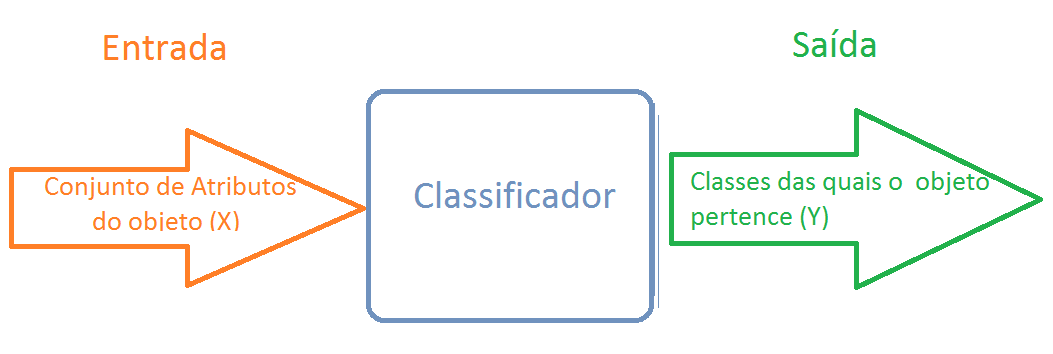
\includegraphics[width=0.9\textwidth]{esquema_classificador.png}
	\caption{Esquema ilustrativo da fun��o de um classificador}
	\label{fig:esquema_classificador}
\end{figure}

\subsection{Classifica��o Bin�ria}

A classifica��o bin�ria � o caso mais simples que pode ser estudado. Neste problema, h� apenas duas classes diferentes e cada objeto pertence a exatamente uma delas. 

Exemplos comuns que podem ser citados s�o a classifica��o de emails em spam ou n�o-spam, a classifica��o de tumores em benignos ou malignos, a determina��o de quais produtos dever�o ser descartados em uma linha de produ��o, a detec��o de transa��es financeiras fraudulentas, etc.

\subsection{Classifica��o \emph{Multi-Class}}
Quando h� mais de duas classes poss�veis, chama-se o problema de classifica��o \emph{multi-class}. Neste caso, cada objeto deve pertencer a exatamente uma dentre as v�rias categorias pr�-definidas. O classificador deve ser capaz de determinar qual � a categoria de cada objeto.

V�rios exemplos de classifica��o podem ser considerados. Dadas imagens de frutas (que podem ser ma��s, peras, ou laranjas) determinar qual � o tipo de cada fruta. Ou ent�o dadas imagens de telesc�pio de galaxias distantes, determinar o tipo da galaxia em quest�o (el�ptica, espiral, etc).

\subsection{Classifica��o \emph{Multi-Class / Multi-Label}}
Quando h� v�rias classes poss�veis (mais de duas) e cada objeto pode pertencer a mais de uma classe, chama-se o problema de \emph{multi-class / multi-label}. Este � o mais dif�cil dos tr�s problemas apresentados, uma vez que h� diversas poss�veis combina��es de classes para cada objeto.

A classifica��o de textos � um cl�ssico exemplo de classifica��o \emph{multi-class / multi-label}, j� que o texto pode pertencer a uma ou varias classes simultaneamente.

Para resolver o problema de classifica��o \emph{multi-class / multi-label} podem ser utilizadas duas abordagens diferentes. Uma delas � a abordagem \emph{one vs all} e a outra � a abordagem dos subconjuntos.

Na abordagem \emph{one vs all}, para cada classe, realiza-se a classifica��o bin�ria do objeto em \emph{pertence} ou \emph{n�o pertence} a esta classe. Desta forma, determina-se todas as classes �s quais o dado objeto pertence. O problema desta abordagem � que pequenos erros que fa�am com que o classificador de uma das classes n�o fique bom (dados ruins para uma classe por exemplo) torna o resultado inteiro ruim.

Na abordagem de subconjuntos, consideram-se todos os poss�veis subconjuntos das classes (com 1, 2, 3, ..., L elementos, onde L � o total de classes) e escolhe-se o subconjunto desejado (utilizando um classificador multi-class). O grande problema desta abordagem � que ha $2^{L - 1}$ poss�veis subconjuntos da classes (o que pode ser muito).

\section{Objeto de Estudo deste Trabalho}
Como foi visto, a classifica��o de textos � um problema do tipo \emph{multi-class / multi-label}, entretanto seria necess�ria uma quantidade muito grande de dados para se obter resultados satisfat�rios neste problema. Portanto, fez-se a simplifica��o de considerar o problema apenas \emph{multi-class}, ou seja, cada texto s� ser� classificado em um �nica classe.
% TODO: Talvez tentar multi class multi label com 1/2/3 classes?



\chapter{Fundamenta��o Te�rica}
\section{Defini��o formal}
Utilizando a nota��o adotada por Dan Jurafsky e Christopher Manning em seu curso de Processamento de Linguagem Natural para Stanford \cite{text_classification}, define-se o problema da classifica��o supervisionada de textos da seguinte forma.

Seja $C=\{c_1, c_2, ..., c_J\}$ um conjunto fixo de classes, $D=\{d_1, d_2, ..., d_n\}$ um conjunto de documentos, e $\mathcal{T}=\{(d_1, c_{d_1}), (d_2, c_{d_2}), ... , (d_m, c_{d_m})\}$ um conjunto de treinamento (subconjunto de $D$) com $m$ documentos classificados manualmente, o classificador consiste em uma fun��o $\gamma :D\rightarrow C$ que relaciona um documento a uma classe, e um algoritmo de aprendizado de m�quina supervisionado � um algoritmo que recebe como par�metros $C$ e $\mathcal{T}$ e retorna $\gamma$.

\section{Tipos de classificadores}
Existem diversos tipos diferentes de classificadores que possuem resultados muito bons dependendo do problema analisado. Segue abaixo uma lista dos principais classificadores existentes.

\begin{itemize}	
	\item �rvores de Decis�o
	\item Na�ve Bayes
	\item Regress�o Log�stica
	\item Support Vector Machines
	\item k-Nearest Neightbors
	\item Redes Neurais
	\item Dentre outros
\end{itemize}

A performance de todos estes m�todos varia consideravelmente dependendo da aplica��o. Estudos mostram que para bases de dados grandes o suficiente, �timos resultados podem ser atingidos independentemente do m�todo utilizado \cite{practical_issues}. Entretanto, para uma quantidade pequena de dados as Na�ve Bayes apresentam resultados bons por serem classificadores de alto \emph{bias} / baixa vari�ncia \cite{quora_classifier}. 

As NB possuem as vantagens de serem f�ceis de se implementar, serem bem r�pidas na hora da execu��o e mostrarem bons resultados pr�ticos.

\section{Redes Bayesianas}

\subsection{Defini��o}
Em modelagem gr�fica probabil�stica, Redes Bayesianas s�o grafos direcionados que representam rela��es de depend�ncia condicionais entre diferentes vari�veis aleat�rias \cite{introduction_to_graphical_models}. A partir da visualiza��o de uma Rede Bayesiana � poss�vel utilizar a regra de Bayes para realizar infer�ncias e descobrir a probabilidade de eventos, dadas algumas vari�veis observadas.As arestas direcionadas representam as no��es de causalidade entre as vari�veis aleat�rias e geram as depend�ncias condicionais. Para cada n� do gr�fico deve haver uma tabela de probabilidades condicionais para a vari�vel em quest�o.

A Figura \ref{fig:bayesian_networks}, retirada do curso de Modelagem Gr�fica Probabil�stica da professora Daphne Koller de Stanford \cite{probabilistic_graphical_models}, ilustra um exemplo de uma Rede Bayesiana simples. Neste caso, pode-se ver que a nota do aluno � influenciada pela dificuldade da prova e pela sua inteligencia. Alem disso A possibilidade do professor escrever uma carta de recomenda��o depende apenas da nota do aluno e o SAT do aluno depende apenas de sua inteligencia. Em cada n� do grafo h� uma tabela de distribui��es de probabilidades condicionais.

\begin{figure}[ht!]
	\centering
	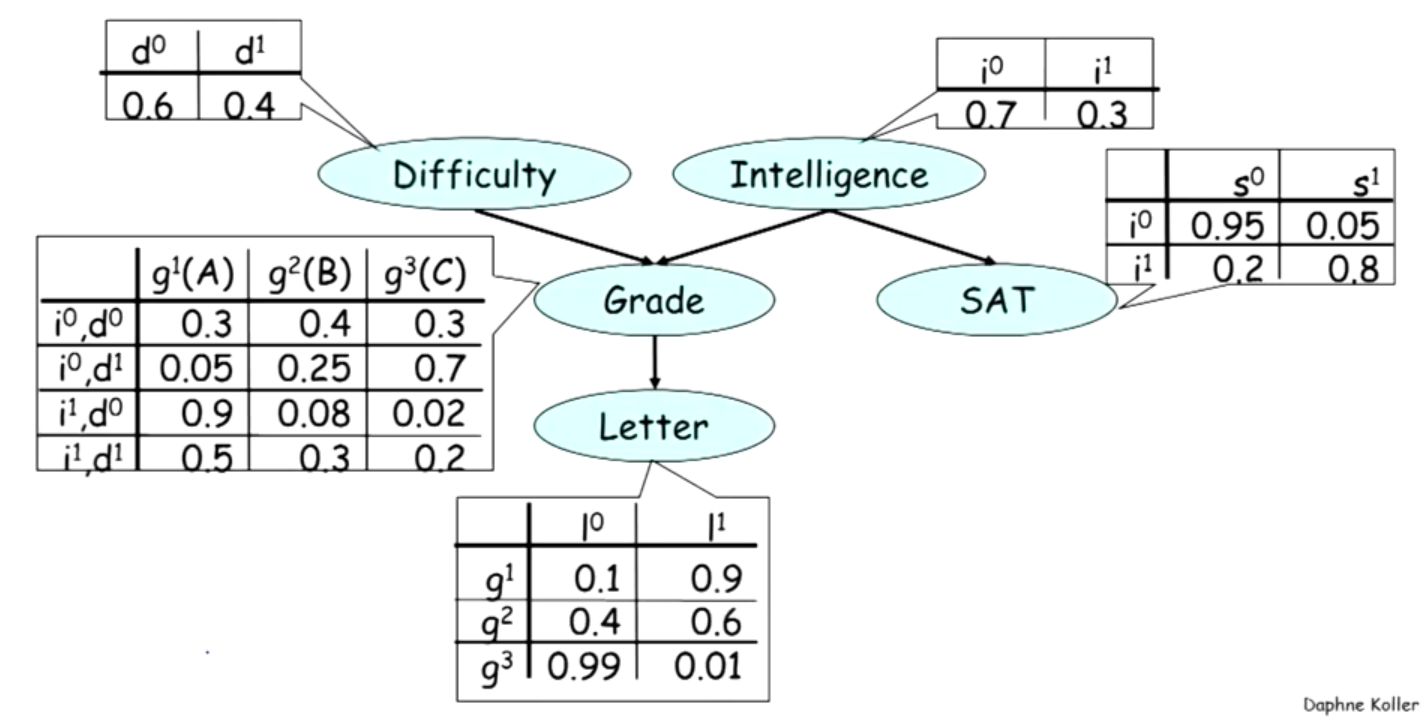
\includegraphics[width=0.9\textwidth]{bayesian_networks.png}
	\caption{Exemplo de Redes Bayesianas}
	\label{fig:bayesian_networks}
\end{figure}


\subsection{Regra de Bayes}
Para realizar infer�ncias nas redes Bayesianas utiliza-se a regra de Bayes, como definida a seguir.

Sejam $A$ e $B$ dois eventos com probabilidades de ocorr�ncia $P(A)$ e $P(B)$ e sendo $P(A|B)$ e $P(B|A)$ as probabilidades condicionais de $A$ dado $B$ e de $B$ dado $A$, respectivamente, tem-se que:

$P(A|B) = \frac{{P(A) P(B|A)}}{P(B)}$

Esse resultado parte da no��o probabilidade conjunta $P(A,B)$.

$P(A,B)=P(A) P(B|A) = P(B) P(A|B) \rightarrow P(A|B) = \frac{{P(A) P(B|A)}}{P(B)}$

No caso do exemplo da Figura \ref{fig:bayesian_networks}, podemos calcular a probabilidade conjunta da rede da seguinte forma:

$P(D,I,G,S,L)=P(D)P(I)P(G|I,D)P(S|I)P(L|G)$ 

Onde $D=Difficulty$, $G=Grade$, $I=Intelligence$, $S=SAT$ e $L=Letter$.

\subsection{Na�ve Bayes}
\subsubsection{Problema a ser resolvido}
Redes Bayesianas s�o ferramentas excelentes para modelar problemas complexos, entretanto elas possuem um grande problema pr�tico. A realiza��o de infer�ncias em redes gen�ricas � um problema NP-hard, conforme demonstrado por Cooper \cite{inference_bayesian_networks}.

O que � realizado na pr�tica �, ou realizar infer�ncias aproximadas nas redes com algoritmos polinomiais, ou simplificar as redes a alguns tipos espec�ficos mais simples.

\subsubsection{O que s�o Na�ve Bayes}
As Na�ve Bayes (bayes ing�nuas) s�o simplifica��es feitas na modelagem de um problema por redes Bayesianas de modo a tornar poss�vel realizar a infer�ncia de forma r�pida. Elas assumem que as vari�veis do problema s�o condicionalmente independentes (mesmo que na pr�tica elas n�o sejam, o que explica o nome \emph{ing�nuas}).

A Figura \ref{fig:naive_bayes_example} mostra um exemplo de uma NB comum. Ela possui uma vari�vel $Classe$ que depende de um s�rie de outras var�veis $x_1, x_2, x_3, ... , x_n$ (que ser�o chamadas a partir daqui de features). � importante notar que a estrutura da rede mostra que as features s�o condicionalmente independentes umas das outras e a $Classe$ depende de cada uma das features individualmente. � f�cil entender a grande vantagem desta abordagem. Cada tabela de probabilidades condicionais ser� pequena. Alem disso a infer�ncia da vari�vel classe, dadas algumas das features ser� bem simples, como ser� mostrado nas pr�ximas se��es.

\begin{figure}[ht!]
	\centering
	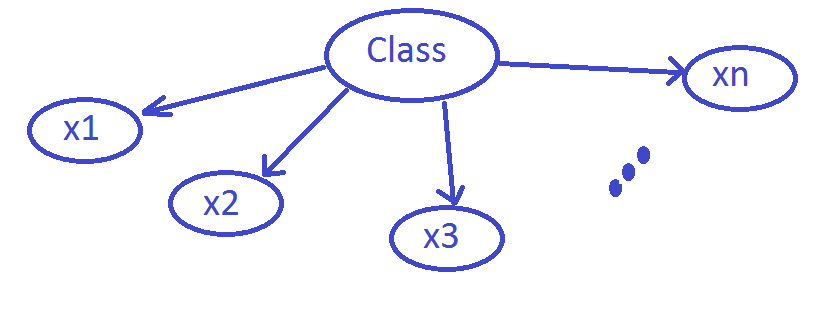
\includegraphics[width=0.9\textwidth]{naive_bayes_example.png}
	\caption{Exemplo de uma Na�ve Bayes}
	\label{fig:naive_bayes_example}
\end{figure}

Na pr�tica o NB � um �timo classificador de textos, pois, al�m de ser simples, traz resultados compar�veis a outros classificadores substancialmente mais complexos e lentos.

\subsubsection{Independ�ncia Condicional}
Antes de explicar a infer�ncia em NB � importante entender o que significa o conceito de independ�ncia condicional.

Dados dois eventos $A$ e $B$, dizemos que eles s�o independentes se a probabilidade de ocorr�ncia de um deles n�o � influenciada pelo fato do outro ter ocorrido. Ou seja:

$P(A|B) = P(A)$
$P(B|A) = P(B)$

Esta propriedade � muito relevante na simplifica��o de express�es pois podemos usar o fato de que a probabilidade conjunta � igual ao produto das probabilidades individuais.

$P(A,B) = P(A)P(B|A) = P(A)P(B)$

\subsubsection{Infer�ncia}
A regra de Bayes seguida pela propriedade de independ�ncia condicional pode ser utilizada para a realiza��o de infer�ncia em NB da seguinte forma.

Sejam $C=\{c_1,c_2,c_3, ..., c_J\}$ um conjunto de classes e $x_1, x_2, x_3, ..., x_n$ as features a serem analisadas. Como trata-se de NB, assume-se independ�ncia condicional das features. Deseja-se saber para cada $i$:

$P(C=c_i|x_1,x_2,...,x_n)$

Ou seja, deseja-se saber qual a probabilidade da classe possuir o valor $c_i$, dadas as features observadas.

Pela regra de Bayes temos:

\begin{equation}
P(C=c_i|x_1,x_2,...,x_n) = \frac{P(x_1,x_2,...,x_n|C=c_i)P(C=c_i)}{P(x_1,x_2,...,x_n)}
\label{eq:bayes_inference}
\end{equation}

Como $x_1, x_2, x_3, ..., x_n$ s�o condicionalmente independentes entre si, temos:


\begin{equation}
\begin{split}
P(x_1,x_2,...,x_n|C=c_i) &= P(x_1,x_2,...,x_{n-1}|x_n,C=c_i)P(x_n|C=c_i) \\ 
&= P(x_1,x_2,...,x_{n-1}|C=c_i)P(x_n|C=c_i) \\
&= P(x_1,x_2,...,x_{n-2}|x_{n-1},C=c_i)P(x_{n-1}|C=c_i)P(x_n|C=c_i) \\
&= P(x_1,x_2,...,x_{n-2}|C=c_i)P(x_{n-1}|C=c_i)P(x_n|C=c_i) \\
&= ... = P(x_1|C=c_i)P(x_2|C=c_i)P(x_3|C=c_i)...P(x_n|C=c_i)  \\
&= \prod_{j=1}^{n}P(x_j|C=c_i)
\end{split}
\label{eq:produtorio}
\end{equation}


Substituindo \ref{eq:produtorio} em \ref{eq:bayes_inference} temos:

\begin{equation}
P(C=c_i|x_1,x_2,...,x_n) = \frac{P(C=c_i)({\prod_{j=1}^{n}P(x_j|C=c_i)})}{P(x_1,x_2,...,x_n)}
\label{eq:naive_bayes_probability}
\end{equation}

\subsubsection{Classifica��o utilizando Na�ve Bayes}
No problema de classifica��o temos um documento $d$ que ser� representado pelas features $x_1,x_2,...,x_n$ e deseja-se saber de qual classe $c \in C$ este documento pertence.

Matematicamente, deseja-se saber de qual classe � mais prov�vel que o documento perten�a. Isto �, a classe que maximiza $P(d|c)$.

$\gamma(d)=argmax_c(P(d|c))=argmax_c(P(x_1,x_2,...,x_n|c))$

Pela equa��o \ref{eq:naive_bayes_probability}, temos que:

$argmax_c(P(x_1,x_2,...,x_n|c)) = argmax_c(\frac{P(C=c_i)({\prod_{j=1}^{n}P(x_j|C=c_i)})}{P(x_1,x_2,...,x_n)})$

Como $P(x_1,x_2,...,x_n)$ n�o depende de c, pode-se cort�-lo do denominador, chegando em:

$\gamma(d) = argmax_c(P(C=c_i)({\prod_{j=1}^{n}P(x_j|C=c_i)})$

Agora, para descobrir a classe do documento, basta calcular $P(C=c_i)$ e $P(x_k|C=c_i)$ e ambas estas probabilidades s�o f�ceis de serem estimadas (se tivermos um conjunto de treino suficientemente grande).

Assumindo que as features sejam binarias, isto �, ou est�o presentes no documento, ou n�o est�o. Seja $\#(x)$ um operador que indica quantas vezes a feature x aparece no conjunto de treinamento e $\#(c)$ quantos documentos do conjunto de treinamento possuem a classe c. Al�m disso, seja $\#(x \wedge c)$ a quantidade de vezes que a feature x aparece num documento de classe c e seja N o total de documentos do conjunto de treinamento. � f�cil ver que:

$P(C=c_i) \simeq \frac{\#(c_i)}{N}$

e

$P(x_j|C=c_i) \simeq \frac{\#(x_j \wedge c_i)}{\#(c_i)}$

Ou seja, o problema de classifica��o se tornou basicamente um problema de contagem.

\subsubsection{Smoothing}
Um dos problemas pr�ticos encontrados por NB � a ocorr�ncia de contagens nulas. O grande problema do 0 � que se ele for apenas um dos fatores da multiplica��o o resultado inteiro ser� 0, inutilizando o m�todo.

Isto n�o � algo incomum, principalmente se o conjunto de treinamento for pequeno. Basta ter uma palavra no conjunto de teste que nunca ocorreu em uma determinada classe no conjunto de treinamento.

Existem t�cnicas que s�o utilizadas para resolver este problema e elas s�o chamadas de Smoothing. Neste trabalho utilizou-se uma das mais comuns: o Laplace Smoothing.

O Laplace consiste em assumir que todas as features foram vistas pelo menos $\alpha$ vezes em cada uma das classes. Isso se traduz nas seguintes formulas, sendo $L$ o n�mero total de classes e $V$ o numero total de features.

$P(C=c_i) \simeq \frac{\#(c_i) + \alpha}{N + \alpha L}$

e

$P(x_j|C=c_i) \simeq \frac{\#(x_j \wedge c_i) + \alpha}{\#(c_i) + \alpha V}$

No caso especial em que $\alpha = 1$, tem-se o \emph{Add-One Smoothing}.

\subsection{Modelagens para classifica��o de texto}
Uma vez que j� foi entendida a forma de classificar o texto, resta apenas represent�-lo por um conjunto de features.

\subsubsection{Na�ve Bayes Bin�ria}
Uma forma comum de representar um texto em features � consider�-lo como um conjunto de palavras. Assume-se que cada palavra � uma feature que pode estar presente ou n�o no documento. Nesta representa��o a ordem das palavras n�o � importante.

Esta representa��o n�o leva em considera��o a frequ�ncia com a qual cada palavra aparece no texto. A f�rmula para calcular a classe mais prov�vel � aquela que foi desenvolvida acima.

% TODO: Continuar essa explica��o

\subsubsection{Na�ve Bayes de Bernoulli}

\subsubsection{Multinomial Na�ve Bayes}
� interessante levar em considera��o a frequ�ncia da ocorr�ncia das palavras uma vez que esta pode trazer informa��o relevante sobre a classe.
% TODO: Entender multinomial bayes e continuar


\subsubsection{Outras features}
� poss�vel enriquecer o classificador utilizando outras features (que n�o sejam as pr�prias palavras do texto). Exemplos de features que podem ser utilizadas s�o: combina��es de palavras, o tamanho do texto, quantidade de sinais de pontua��o, quantidade de palavras com iniciais mai�sculas, etc.

Para o caso espec�fico de postagens em redes sociais existem ainda outras features que podem ser inclu�das. Pode-se considerar o autor da postagem, o momento em que ela foi publicada, a presen�a de fotos, v�deos ou links, etc.

\section{Weighted Na�ve Bayes}
Um dos problemas das NB � que muitas vezes nas aplica��es reais n�o � poss�vel assumir a independ�ncia condicional das features. Muitas vezes uma das features tem um peso maior que as outras, por exemplo.

Um modo inicial de relaxar essa hip�tese de independ�ncia, � eliminar features com alta correla��o, fazendo com que o subconjunto restante se encaixe melhor na hip�tese de independ�ncia condicional. Isto � chamado de sele��o de features.

Neste caso temos:

$\gamma(d) = argmax_c(P(C=c_i)({\prod_{j=1}^{n}P(x_j|C=c_i)^{I(j)}})$

Onde:

$I(j) \in \{0,1\}$

Uma abordagem mais gen�rica � ponderar cada feature de acordo com sua relev�ncia. Ou seja:

$\gamma(d) = argmax_c(P(C=c_i)({\prod_{j=1}^{n}P(x_j|C=c_i)^{w(j)}})$

Onde:

$w(j) \in \mathbb{R}^+$

Nota-se que a sele��o de features � um caso espec�fico da pondera��o de features (onde $w(j)$ s� pode ser 0 ou 1).

Agora o grande problema passa a ser determinar os pesos $w(j)$ das features. H� diversos algoritmos que ja foram propostos para realizar esta tarefa.

% TODO: Escrever sobre outros approachs the feature weighting (tem naquele artigo)

Neste trabalho, estudou-se a utiliza��o de um m�todo baseado na Teoria da Informa��o, que al�m de ser comum na literatura, possui fundamentos te�ricos bem embasados \cite{weighted_naive_bayes}. 

% TODO: Escrever sobre feature weighting


\section{M�todos de avalia��o de um classificador}
Uma vez desenvolvido o classificador � importante ser capaz de avali�-lo a fim de determinar o qu�o bom ele �. A utiliza��o de m�tricas num�ricas para avaliar os classificadores � interessante pois permite a realiza��o de compara��es entre as diferentes vers�es implementadas, tornando poss�vel determinar se as modifica��es que foram feitas est�o fazendo efeito.

Existem diversas m�tricas que podem ser utilizadas para avaliar classificadores, algumas delas ser�o analisadas nesta se��o.

\subsection{Classificador Bin�rio}

\subsubsection{Acur�cia}

\subsubsection{Precis�o}

\subsubsection{Abrang�ncia (\emph{Recall})}

\subsubsection{Medida F1}

\subsection{Classificador \emph{Multi-Class}}

\subsubsection{Matriz de Confus�o (\emph{Confusion Matrix})}

\subsubsection{M�dias micro e macro (\emph{Micro and Macro Averaging})}

\subsubsection{Medida Kappa}





\chapter{Metodologia}
\section{Plano de desenvolvimento}

Dividiu-se o desenvolvimento do projeto em diversas etapas.

\subsection{Estudo basico sobre Processamento de Linguagem Natural}
Inicialmente realizou-se um estudo aprofundado sobre o assunto do projeto para aproveitar o conhecimento j� desenvolvido ao longo dos anos pela comunidade cient�fica e garantir que as melhores tecnologias e t�cnicas fossem adotadas.
O plano de estudos adotado foi:

\begin{enumerate}[(a)]
\item Express�es regulares
\item Processamento de texto
\item Normaliza��o
\item Tokeniza��o das strings
\item Modelagem lingu�stica e simplifica��o de N-gramas
\item Classifica��o de texto
\item Na�ve Bayes
\item M�tricas de performance (Precis�o, Abrang�ncia, Acur�cia, etc)
\item Melhorias para Na�ve Bayes
\end{enumerate}

\subsection{Coleta de dados}
Como trata-se de um projeto de Intelig�ncia Artificial, � essencial que se obtenha uma base de dados grande o suficiente para que o sistema desenvolvido seja capaz de realizar as generaliza��es necess�rias para um bom funcionamento sem que haja overfit.

Esta base de dados consiste em um conjunto de postagens (vari�vel X) e o assunto da mesma (vari�vel Y).

Foram propostas duas formas poss�veis de aquisi��o de dados.

\begin{itemize}
\item Uma delas foi desenvolver um plugin que colete as postagens e pergunte o assunto para o usu�rio. A utiliza��o deste plugin por v�rias pessoas permitiu a aquisi��o de uma base de dados consider�vel.
\item Paralelamente desenvolveram-se crawlers para vasculhar sites que contenham artigos e textos sobre cada assunto que se deseja classificar. � importante ter a capacidade de classificar artigos de sites gen�ricos, pois muitas das postagens em rede social possuem links para tais sites.
\end{itemize}

\subsection{Pr�-processamento dos textos e normaliza��o}
Como trata-se de linguagem natural e ainda por cima coloquial, para atingir um bom resultado com o classificador � essencial que haja um bom pr�-processamento do texto corrigindo palavras erradas, frases mal-constru�das, normalizando termos parecidos, etc.


\subsection{Cria��o dos classificadores de Redes Bayesianas}
Foram criados classificadores de NB e suas performances foram avaliadas contra um conjunto de valida��o. Os m�todos mais efetivos foram selecionados, combinando os classificadores de postagens e de artigos e ajustando seus par�metros para obter um bom resultado final.

\subsection{Estudo dos resultados obtidos no conjunto de valida��o para diferentes features e par�metros}
\label{sec:validacao}
Foi realizado um estudo detalhado dos resultados obtidos pelos classificadores para diferentes features, par�metros e t�cnicas de classifica��o (NB e NB com pesos). A avalia��o final da rede foi realizada em um conjunto de teste separado. 

Separou-se a base de dados total em dois conjuntos. Um de treinamento e um de valida��o de forma aleat�ria, sendo 25\% para valida��o e 75\% para treinamento. Para a an�lise da qualidade do classificador realizou-se a m�dia das estat�sticas avaliadas para varias divis�es aleat�rias diferentes de modo a obter um resultado est�vel.

\subsection{Defini��o da arquitetura do classificador e sua implementa��o}
Definiu-se que a rede seria treinada e armazenada em um servidor central. Considerou-se tamb�m a possibilidade da rede ser din�mica (ou seja, se a intera��o com o usu�rio fazer com
que a rede aprenda online com as novas informa��es).

\subsection{Desenvolvimento do plugin}
Por fim desenvolveu-se o plugin para o Google Chrome, com uma interface gr�fica amig�vel para o usu�rio para que ele entenda de forma f�cil como filtrar as postagens em seu feed de not�cias. %TODO: Nao fizemos isto ainda

\subsection{Testes de usabilidade}
% TODO: Tirar isso daqui?
Por fim foram realizados testes de usabilidade com colegas de turma baseados nas heur�sticas de Nielsen.


\section{Aquisi��o de dados}
Como j� foi dito, foram desenvolvidas duas formas diferente de realizar a aquisi��o de dados. Uma delas consiste numa extens�o para o Google Chrome que possibilita o usu�rio classificar cada postagens � qual ele se depara no Facebook, enviando os dados e a classifica��o da mesma para o banco de dados. A outra forma de aquisi��o de dados � o desenvolvimento de um crawler que faz o download diversos artigos online.

\subsection{Extens�o do Chrome de classifica��o de postagens}
\label{sec:plugin_chrome}
\subsubsection{Funcionamento de extens�es do Chrome}
Extens�es s�o softwares que melhoram as funcionalidades de um navegador. O Google Chrome disponibiliza um Framework de desenvolvimento de extens�es com muitas capacidades \cite{chrome_extension}.

A extens�o consiste em um conjuntos de arquivos zipados que incluem HTML, Javascript, CSS, imagens, etc. O Javascript de uma extens�o pode ser dividido em 3 partes diferentes: c�digo de extens�o (\emph{extension code}), scripts de conte�do (\emph{content scripts}) e scripts injetados (\emph{injected scripts}). Estes tr�s modos foram descritos abaixo.

\begin{itemize}
\item \textbf{C�digo de extens�o:} Trata-se do c�digo injetado diretamente no browser, tendo portanto acesso a todas as funcionalidades da API do Chrome, como tabs de background, pop-ups do navegador (aqueles pequenos �cones das extens�es que ficam no canto superior direito do chrome), etc.

\item \textbf{Scripts de conte�do:} Trata-se de um c�digo que � executado quando uma determinada p�gina � carregada pelo usu�rio. Este script possui um escopo entre o do c�digo de extens�o e o do script injetado. Os scripts de conte�do t�m acesso � algumas das funcionalidades da API do Chrome e ao mesmo tempo pode acessar e modificar o DOM da p�gina. Por estar em um escopo diferente ao escopo do javascript da pr�pria p�gina ele n�o tem acesso �s fun��es e objetos definidos no mesmo. Por outro lado, ele n�o possui diversas das restri��es de seguran�a que scripts injetados possuem. O script de conte�do pode, por exemplo, executar cross-origin requests (ou seja, acessar servidores de outra origem).

\item \textbf{Scripts injetados:} Scripts injetados s�o, como o nome diz, peda�os de c�digo javascript que s�o injetados numa determinada p�gina, executando em seu escopo. Desta forma eles tem acesso � todas as fun��es e vari�veis definidos pelo javascript original da p�gina. Tamb�m podem modificar como eles quiserem estas vari�veis e o pr�prio DOM.

\end{itemize}

No caso da aplica��o deste trabalho, � necess�rio ser capaz de mandar os dados das postagens com suas classifica��es para um servidor central (que obviamente n�o � do pr�prio Facebook), logo scripts injetados n�o s�o uma boa solu��o (uma vez que o javascript do Facebook impede a execu��o de cross-origin requests). Ou seja, a extens�o foi desenvolvida predominantemente com scripts de conte�do. 

Uma observa��o importante � que scripts de conte�do ainda possuem algumas restri��es de seguran�a ao fazer requests para outros dom�nios. Se o site principal for https, o script de conte�do s� poder� realizar requests para outros servidores por https tamb�m. Para tal, o servidor desenvolvido neste trabalho deve ser capaz de responder requests https.

\subsubsection{Manifesto da extens�o}
As extens�es do Chrome possuem um arquivo de configura��o chamado de manifesto. Este arquivo encontra-se no formato de JSON.

\begin{lstlisting}[language=json, firstnumber=1, caption={Manifesto da extens�o do Chrome para coleta de dados}, label={lst:manifest_chrome_extension}]
{
  "manifest_version": 2,
  "name": "Demeter",
  "version": "1.0.0",
  "description": "Collect data from facebook to use in NLP studies. This plugin has academic purposes.",

  "icons": {
    "128" : "icon_128.png",
    "180" : "icon_180.png"
  },

  "content_scripts": [{
    "matches": [ "https://*.facebook.com/*" ],
    "js": [ 
      "jquery-1.11.3.min.js", 
      "poo_utilities.js",
      "facebook_tree.js",
      "demeter_dom.js",
      "story_classification.js",
      "contentscript.js" 
    ],
    "css": [ "demeter.css" ]
  }],

  "permissions": [ "tabs", "https://*.facebook.com/*", "https://demeter-1075.appspot.com/*" ],

  "web_accessible_resources": [ 
    "contentscript.js", 
    "jquery-1.11.3.min.js", 
    "poo_utilities.js", 
    "facebook_tree.js",
    "story_classification.js",
    "demeter_dom.js",
    "demeter.css",
    "three-dots.png"
  ]
}

\end{lstlisting}

O c�digo \ref{lst:manifest_chrome_extension} ilustra o manifesto da extens�o desenvolvida. Ele identifica o nome da extens�o (Demeter), a sua vers�o, os �cones utilizados, os scripts de conte�do e as permiss�es (acessar o facebook e o servidor desenvolvido).

Note que al�m dos c�digos desenvolvidos, utilizou-se a biblioteca do JQuery para facilitar a manipula��o do DOM.

\subsubsection{Estrutura do DOM do Facebook}
Para injetar um peda�o de HTML no meio do Feed de not�cias do Facebook, � importante entender a sua estrutura, b�sica. 

Este projeto foi feito assumindo que o Facebook n�o iria realizar grandes mudan�as em seu design e em sua estrutura b�sica de HTML em um curto prazo. Caso houvesse tal modifica��o, a extens�o desenvolvida iria parar de funcionar, sendo necess�rio realizar algumas adapta��es para que ela fosse consertada. Todo c�digo foi desenvolvido de forma modularizada de modo a tentar diminuir as dificuldades de adapta��o caso este evento infort�nio ocorresse. Todavia, desde o come�o at� o final do desenvolvimento do projeto isto n�o aconteceu.

O HTML do Facebook passa por um processo de ofusca��o e compress�o antes de ser enviado para as m�quinas cliente. Essa ofusca��o troca as classes e ids dos elementos por nomes aleat�rios e curtos. Ent�o um elemento HTML que originalmente tinha uma classe `facebook{\_}feed', por exemplo, passar� a ter a classe `{\_}u{\_}s8v4'. Este processo atrapalha um pouco no desenvolvimento de uma extens�o que se acople ao site do Facebook (pois esses ids e classes s�o aleat�rios e podem mudar). Entretanto, por algum motivo (provavelmente se trata de um c�digo antigo), algumas classes e ids continuam com nomes leg�veis. Considerou-se que estes nomes leg�veis s�o mais est�veis e portanto, baseou-se a extens�o desenvolvida em elementos HTML que possu�am estes nomes.

\begin{figure}[ht!]
	\centering
	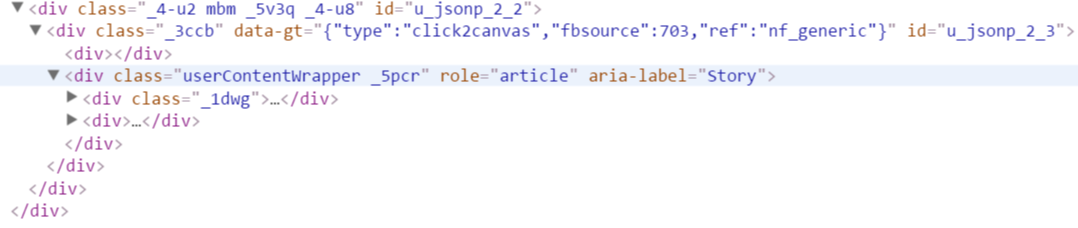
\includegraphics[width=0.9\textwidth]{facebook_html_example.png}
	\caption{Exemplo de HTML do Facebook, com algumas classes aleat�rias e algumas de nome leg�vel}
	\label{fig:facebook_html_example}
\end{figure}

A Figura \ref{fig:facebook_html_example} ilustra o que foi explicado no par�grafo anterior. Algumas das classes s�o strings aleat�rias(`{\_}5pcr', `{\_}3ccb', `{\_}1dwg', etc), enquanto que algumas possuem valores leg�veis (`userContentWrapper').

Observando estes elementos nomeados, chegou-se � seguinte estrutura simplificada para o DOM do Facebook. Todo o conte�do do site, exceto a barra azul superior e o chat que fica ao lado direito, se encontra dentro de um div chamado de mainContainer. Dentro deste mainContainer h� um div chamado de feed{\_}stream, que possui todas as postagens do feed de not�cias. O feed{\_}stream contem um ou mais substreams. Cada substream � um conjunto de postagens. Quando o usu�rio desce a p�gina at� a parte inferior, um novo substream � criado com as novas postagens. Cada substream possui uma ou mais postagens que s�o representadas por divs chamados de userContentWrapper. � poss�vel que userContentWrapper's contenham outros userContentWrapper's (por exemplo quando uma pessoa compartilha a postagem de outra pessoa). A Figura \ref{fig:facebook_dom_structure} mostra um exemplo de uma �rvore de DOM simplificada para o Facebook.

\begin{figure}[ht!]
	\centering
	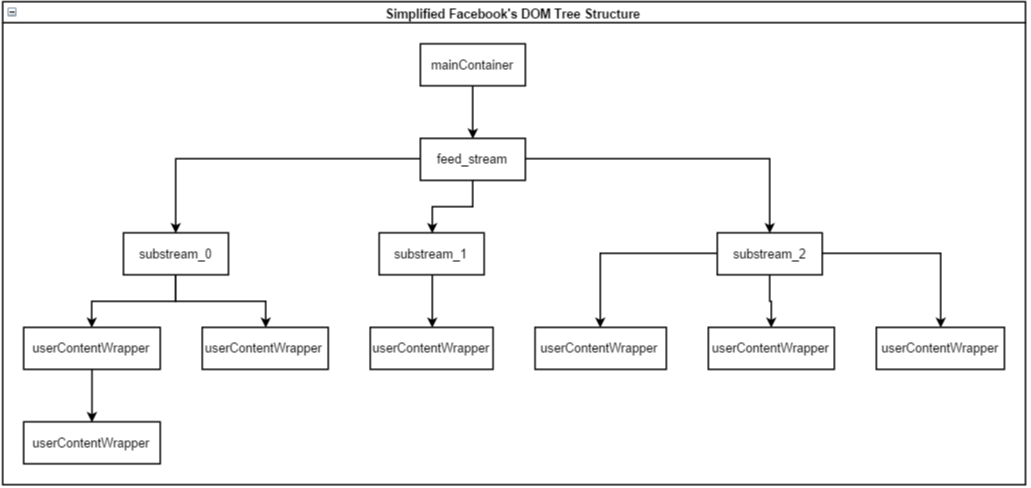
\includegraphics[width=0.9\textwidth]{facebook_dom_structure.png}
	\caption{Exemplo ilustrativo da estrutura b�sica da �rvore de DOM do Facebook}
	\label{fig:facebook_dom_structure}
\end{figure}

\subsubsection{UI desenvolvida}
A extens�o desenvolvida utiliza a API de javascript JQuery para injetar um peda�o de HTML logo acima do userContentWrapper, de modo a colocar um cabe�alho no topo de cada postagem com as classes pr� definidas. O usu�rio dever� agir como um supervisor para o classificador indicando qual o assunto da postagem em quest�o. A Figura \ref{fig:chrome_extension_header_example} ilustra o cabe�alho em uma postagem.

\begin{figure}[ht!]
	\centering
	
\includegraphics[width=0.9\textwidth]{chrome_extension_header_example.png}
	\caption{Exemplo em uma postagem do cabe�alho contendo as poss�veis classes}
	\label{fig:chrome_extension_header_example}
\end{figure}

Uma vez que o usu�rio clique na classe � qual a postagem pertence, o cabe�alho passa a conter apenas o nome da classe escolhida e uma barra op��es a direita que pode ser expandida, conforme a Figura \ref{fig:chrome_extension_header_classified}

\begin{figure}[ht!]
	\centering
	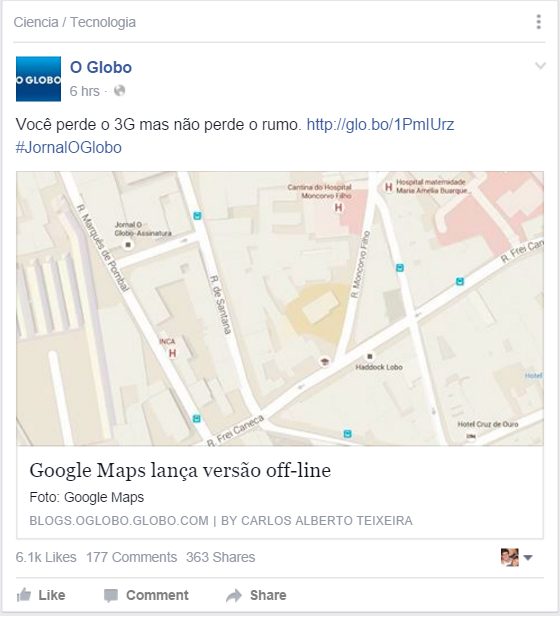
\includegraphics[width=0.9\textwidth]{chrome_extension_header_classified.png}
	\caption{Exemplo da UI de uma postagem classificada pelo usu�rio}
	\label{fig:chrome_extension_header_classified}
\end{figure}

A barra de op��es possui duas poss�veis a��es: `Mudar Assunto' ou `Adicionar Assunto'. Se o usu�rio clicar na primeira op��o ele poder� escolher um novo assunto para a postagem. Se o usu�rio clicar na segunda op��o ele poder� adicionar um novo assunto para a postagem (que ent�o possuir� duas classes). A Figura \ref{fig:barra_de_opcoes_extencao} ilustra a barra de op��es.

\begin{figure}[ht!]
	\centering
	
\includegraphics[width=0.9\textwidth]{barra_de_opcoes_extencao.png}
	\caption{Barra de op��es para modificar a escolha do assunto na extens�o do Chrome}
	\label{fig:barra_de_opcoes_extencao}
\end{figure}

Observe que apesar de na hora de realizar a classifica��o foi feita a simplifica��o de que o problema se trata apenas de \emph{multi-class} (n�o \emph{multi-class / multi-label}), na hora da coleta de dados � poss�vel classificar uma �nica postagem em v�rios assuntos diferentes. Isto foi feito primordialmente por dois motivos. Primeiramente, � interessante j� possuir uma base de dados com postagens com classifica��es m�ltiplas para se poder estudar o classificador \emph{multi-class / multi-label} em trabalhos futuros. Al�m disto, v�rios usu�rios diferentes podem classificar as postagens de forma distinta (n�o concordam entre si). Neste caso, o servidor guarda a contagem de classifica��es para cada classe e � considerado que a postagem pertence � classe mais frequente (empates s�o quebrados manualmente).

\subsubsection{Servidor}
Sempre que um usu�rio seleciona uma classe para uma determinada postagem, � realizada uma requisi��o POST para o servidor do Demeter (nome do projeto), contendo as informa��es relevantes. O servidor salva estas informa��es em um banco de dados.

O banco de dados contem postagens indexadas por sua url (que � um valor �nico para cada postagem) e � associado a um conjunto de classes e frequ�ncias. Por exemplo, se um post foi classificado 5 vezes como Pol�tica e 2 como educa��o, essa informa��o ficar� registrada no banco de dados.

� importante notar que n�o � apenas o texto da postagem que � salva no banco de dados. Tamb�m armazena-se o usu�rio que realizou criou a postagem, o momento em que ela foi publicada (timestamp), a presen�a de fotos ou v�deos, a exist�ncia de informa��es sobre o local de onde o usu�rio postou, etc. Essas informa��es podem ser relevantes na hora de se criar features para a NB.


\subsubsection{Crawler}

% TODO: Write about crawler

\section{Processamento do texto}
\label{sec:processamento_do_texto}

Um bom pr� processamento do texto � essencial para um bom resultado de classifica��o. Isso � especificamente v�lido em um ambiente como uma rede social, onde muitas vezes h� abrevia��es, interjei��es, utiliza��o de linguagem informal, etc.

\subsection{Tokeniza��o}
Muitas vezes as palavras puras n�o s�o muito boas para utilizar como features na classifica��o. Por isso para cada palavra associa-se um token. Este processo � chamado de tokeniza��o. Deve-se decidir o que ser� feito com a pontua��o, se palavras ser�o modificadas, etc. As vezes um token pode ser um conjunto de palavras. Por exemplo `Rio de Janeiro' pode ser um �nico token.

Outros exemplos de tokeniza��o s�o trocar todos os n�meros por um �nico token (normalmente para um classificador n�o � t�o importante o valor num�rico, mas sim a presen�a de um n�mero em si). O mesmo vale para datas, porcentagens, links, etc.

\subsection{Normaliza��o}
Normaliza��o � o processo de se criar classes de equival�ncia de palavras. Por exemplo: as palavras U.S.A e USA s�o a mesma, por�m escritas de forma diferente. Alem disso palavras possuem a primeira letra mai�scula quando iniciam uma frase ou podem estar completamente escritas em caixa alta (se o escritor quer passar a no��o de que est� gritando, por exemplo). Transformar todas as letras para caixa baixa � um tipo de normaliza��o.

\subsection{Stemming}
Stemming � o processo de trocar todas as palavras que possuem sentidos parecidos por um mesmo radical. Por exemplo, os verbos escrevo, escrevi, escrevemos, escreverei, escrevera e escreveu podem ser substitu�dos pelo radicar escrev.

\subsection{Processamento utilizado}

%TODO: Se implementarmos stemming ele tem que entrar nessa secao
Para este trabalho foram feitas as seguintes etapas de pr� processamento do texto.

\begin{itemize}
\item \textbf{Remover caracteres unicode:} Acentos, cedilhas, tremas e outros caracteres unicode s�o substitu�dos por seus equivalentes em ASCII.
\item \textbf{Remover letras mai�scula:} Todas as letras mai�sculas s�o mudadas para min�scula.
\item \textbf{Remo��o n�meros:} Quando h� um n�mero no texto, seu valor exato n�o importa muito para o classificador. O que importa � a sua presen�a. O mesmo vale para datas, porcentagens, urls, valores de dinheiro e datas. No caso, os n�meros s�o substitu�dos por `\{number\}', as datas por `\{date\}' e assim por diante.
\item \textbf{Remover a pontua��o:} Toda a pontua��o � removida.
\item \textbf{Encontrar risadas:} Todas as ocorr�ncias de risadas (que puderam ser identificadas com algumas heur�sticas simples) s�o substitu�das por `{laughter}'
\item \textbf{Remover letras duplas:} Em redes sociais � muito comum o usu�rio repetir a mesma letras diversas vezes para enfatizar a palavra. Por exemplo: `Que FOOOOOOOOOOFO!'. Isto atrapalharia o classificador. Por isso letras repetidas s�o removidas. Note que, apesar de ser permitido no portugu�s `r' e `s' duplos, remov�-los n�o atrapalhar� muito o classificador.
\item \textbf{Filtrar palavras comuns e que n�o agregam muito valor ao classificador:} Palavras comuns do portugu�s como artigos, preposi��es, etc, s�o desconsideradas.
\end{itemize} 

\section{Tecnologias utilizadas}

Para o desenvolvimento deste projeto, foram utilizadas diversas tecnologias e ferramentas computacionais diferentes.

O versionamento de c�digo foi feito utilizando o Git, com reposit�rio p�blico hospedado no Github.

Para se desenvolver a extens�o do Chrome utilizou-se o framework disponibilizado pelo pr�prio Google. As linguagens adotadas para tal foram Javascript, HTML e CSS.

O servidor foi feito no Google App Engine, que permite a utiliza��o da infraestrutura do Google de forma gratuita e simples. O utilizou-se a API do NDB para o gerenciamento do banco de dados.

O classificador foi inteiramente desenvolvido em Python 2.7 por conta de sua versatilidade e facilidade de programa��o.


\chapter{Propostas de Classificadores}
\label{sec:proposta_de_classificador}

\externaldocument{fundamentacao_teorica}
\externaldocument{metodologia}

Foram propostas diversas formas diferentes de classificadores, e cada uma ser� posteriormente avaliada e comparada.

\section{Classes adotadas}
\label{ref:classes_adotadas}
Foram consideradas as seguintes classes para todos os classificadores desenvolvidos:

\begin{itemize}
	\item Politica / Economia 
	\item Propaganda
	\item Filmes / Series
	\item Humor
	\item Celebridade
	\item Esporte
	\item Pessoal
	\item Turismo
	\item Ciencia / Tecnologia / Meio Ambiente
	\item Minorias
	\item Educacao
	\item Noticias
	\item Bebes / Animais
	\item Saude
\end{itemize}

\section{Na�ve Bayes utilizando apenas o texto}
O classificador mais simples que pode ser criado utilizando NB, consiste em utilizar apenas as palavras do texto como features. 

Neste caso, realizou-se primeiramente o processamento conforme o descrito na Se��o \ref{sec:processamento_do_texto}, normalizando as palavras de forma apropriada. Durante o processo de normaliza��o, foram realizadas as seguintes modifica��es.

\begin{itemize}
	\item Todos os links foram trocados pelo token '\{link\}'
	\item Todas as refer�ncias feitas com @ (por exemplo @NomeDaPessoa) foram trocadas pelo token '\{tag\}'
	\item Todos os valores monet�rios (tanto em real como em d�lar) foram trocados pelo token '{money}'
	\item Todas as percentagens foram trocadas pelo token '\{percentage\}'
	\item Todas as datas foram trocadas pelo token '\{date\}'
	\item Todos os outros n�meros foram trocados pelo token '\{number\}'
\end{itemize}

Em seguida, realizou-se o treinamento utilizando base de dados obtida, realizando-se a contagem da ocorr�ncia dos tokens em cada uma das classes. Finalmente testou-se a performance do classificador obtido em um conjunto de testes.

\section{Na�ve Bayes com Features Adicionais}
\label{sec:bayes_features_adicionais}
V�rias outras features foram adicionadas na tentativa de melhorar a performance do classificador. As postagens em redes sociais em geral contem muito mais informa��es do que o texto escrito. Tentaram-se captur�-las utilizando as seguintes features:

\begin{itemize}
	\item Usu�rio ou p�gina que � autor(a) da postagem
	\item Tipo de compartilhamento (se � apenas um status update, ou se � um v�deo ou uma foto que est�o sendo compartilhados)
	\item Se a postagem possui uma localiza��o de origem (o valor do local em si de onde a postagem foi feita n�o foi considerado, pois seria necess�ria uma base de dados muito grande para que este local fizesse diferen�a)
	\item Se h� algum outro usu�rio marcado na postagem (considerou-se esta feature interessante pelo fato de que postagens pessoas costumam ter pessoas marcadas).
	\item Se a postagem foi promovida por meio de pagamentos (tem a tag Sponsor no Facebook) ou n�o
	\item O tamanho do texto (discretizou-se o tamanho em 4 categorias: tiny, small, medium, large)
\end{itemize}

� importante notar que o ideal seria recuperar informa��es a partir das imagens e v�deos compartilhados, entretanto este problema foge ao escopo deste trabalho.



\section{Weighted Na�ve Bayes utilizando apenas o texto}
Utilizaram-se as Weighted Na�ve Bayes descritas na Se��o \ref{sec:weighted_naive_bayes} para ponderar a import�ncia das features relevando a no��o independ�ncia condicional das NBs.

\section{Weighted Na�ve Bayes com Features Adicionais}

Repetiu-se a mesma ideia exposta na Se��o \ref{sec:bayes_features_adicionais}, porem desta vez com a NB ponderada.

\section{Utiliza��o dos links}
At� agora, o conte�do dos links compartilhados tinha sido completamente ignorado. Por exemplo, se algu�m postasse um link sobre economia e escrevesse algo do tipo `Muito interessante esta an�lise', o classificador iria tentar classificar a potagem utilizando apenas o texto (o que � bem complicado). Para evitar este problema, fez-se um HTTP GET request para o link, extraiu-se o texto principal e ele foi classificado por um segundo classificador. O resultado deste segundo classificador passa a ser uma feature do classificador de postagens.

Este segundo classificador (que ser� referenciado como classificador de artigos) foi treinado a partir da base de dados adquirida pelo crawler.
 
\section{Concatena��o do texto dos links}
% TODO: Falar da concatena��o do texto dos links no post (se a gente efetivamente fizer isto)
% Uma outra abordagem utilizada foi a de concatenar o texto contido no link com o texto da postagem. Desta forma ambos s�o treinados e classificados simultaneamente.

\section{Fus�o de classes pequenas}
% TODO: Falar das classes pouco frequentes
% Uma outra mudan�a considerada para melhorar a qualidade do classificador foi a fus�o de classes pequenas.

% Muitas das classes consideradas n�o s�o t�o recorrentes no Facebook dos supervisores e portanto conseguiram poucos exemplos para os conjuntos de treinamento e teste. Isto faz com que o classificador n�o possua informa��o suficiente para realizar a classifica��o de forma adequada.

% Al�m disso, existem algumas classes que possuem dom�nios bem proximos que, muitas vezes, s�o de dif�cil distin��o at� para um ser humado (cita-se como exemplo `Celebridades' vs `Filmes'). Isto tambem aumenta a taxa de errodo classificador.

% A solu��o adotada foi a fus�o destas classes em outra mais abrangentes.


\chapter{Valida��o - Experimentos, resultados e an�lise}
\externaldocument{metodologia}
\externaldocument{fundamentacao_teorica}
\externaldocument{proposta_de_classificador}

\section{Base de dados}
A base de dados para a classifica��o de postagens foi adquirida a partir da extens�o do Chrome descrita na Se��o \ref{sec:plugin_chrome}. A classifica��o foi feita manualmente por diversos supervisores, classificando cada postagem nas diferentes categorias explicitadas na Se��o \ref{ref:classes_adotadas}. 

O gr�fico da Figura \ref{fig:classes_freq} ilustra a propor��o entre as diferentes classes na base de dados obtida.

\begin{figure}[ht!]
	\centering
	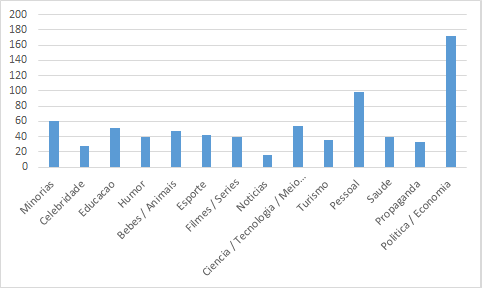
\includegraphics[width=0.9\textwidth]{classes_freq.png}
	\caption{Histograma representativo da base de dados de postagens adquirida}
	\label{fig:classes_freq}
\end{figure}

A menor base � de `Not�cias', com apenas 16 postagens, e a maior � `Pol�tica / Economia' com 172 postagens. O total de postagens � 757. Observa-se que este n�o � um n�mero muito grande para uma base de dados, ainda mais com um total de 14 classes, mas foi o que foi poss�vel de se adquirir.

\section{Na�ve Bayes utilizando apenas o texto}

Nesta primeira abordagem, o classificador obteve uma acur�cia m�dia (ao longo de 100 parti��es aleat�rias diferentes da base de dados em treinamento e valida��o, conforme o explicado na Se��o \ref{sec:validacao}) de 49.7\%, ou seja, o classificador acerta basicamente 1 a cada 2 postagens. Como j� foi dito na Se��o \ref{sec:acuracia}, a acur�cia � uma m�trica bem ruim para avaliar um classifiador. Desta forma, foram consideradas as outras estat�sticas explicadas no cap�tulo de metodologia, para uma an�lise mais profunda.

A acur�cia esperada para este classificador, utilizando a Equa��o \ref{eq:acuracia_esperada}, � de 14.16\%. O $Kappa$ neste caso foi de 41.4\%. Segundo o benchmark de Landis e Koch \cite{landis1977measurement}, trata-se de um resultado moderado. Note que a estat�stica $Kappa$ agrega muito mais informa��o que uma simples acur�cia.

� interessante observar como o Kappa e a acur�cia variam conforme se aumenta o tamanho da base de dado. Para tal, repetiu-se o processo de treinamento e valida��o com a base de dados de tamanho vari�vel (pegando-se subconjuntos aleat�rios da base de dados original). Manteve-se sempre uma propor��o de 75\% pra treinamento e 25\% para valida��o. A Figura \ref{fig:nb_apenas_com_texto_accuracy_graph} mostra o crescimento da acur�cia, enquanto que a Figura \ref{fig:nb_apenas_com_texto_kappa_graph} mostra o crescimento do Kappa.

\begin{figure}[ht!]
	\centering	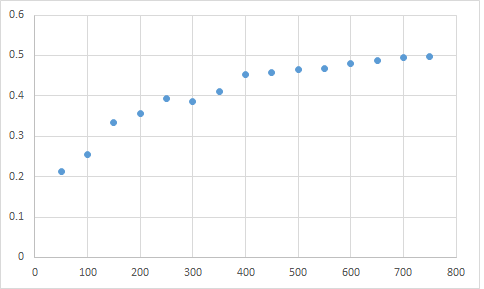
\includegraphics[width=0.9\textwidth]{nb_apenas_com_texto_accuracy_graph.png}
	\caption{Acur�cia em fun��o da quantidade de postagens na base de dados (treinamento + valida��o) para NB simples}
	\label{fig:nb_apenas_com_texto_accuracy_graph}
\end{figure}

\begin{figure}[ht!]
	\centering	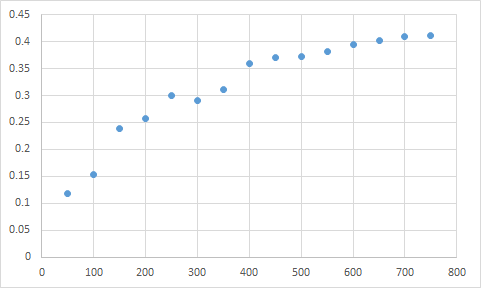
\includegraphics[width=0.9\textwidth]{nb_apenas_com_texto_kappa_graph.png}
	\caption{Kappa em fun��o da quantidade de postagens na base de dados (treinamento + valida��o) para NB simples}
	\label{fig:nb_apenas_com_texto_kappa_graph}
\end{figure}

Para se compreender onde exatamente o classificador est� ruim, rodou-se novamente o programa com apenas uma itera��o e construiu-se a matriz de confus�o para os resultados obtidos, como pode ser visto na Tabela \ref{tab:nb_apenas_com_o_texto}.

Para este exemplo tem-se:

$acuracia=0.529101$

$acuracia\_esperada=0.138154$

$Kappa=0.453615$


A Tabela \ref{tab:nb_apenas_com_o_texto} apresenta a matriz de confusao.


\begin{table}[tph]
	\begin{center}
		\begin{tabular}{ c  c  c  c  c  c  c  c  c  c  c  c  c  c }
			\hline
			Beb & Cel & Cie & Edu & Esp & Fil & Hum & Min & Not & Pes & Pol & Pro & Sau & Tur\\
			\hline
			7 & 0 & 1 & 0 & 0 & 0 & 0 & 0 & 0 & 1 & 0 & 2 & 0 & 0\\
			0 & 1 & 0 & 0 & 0 & 1 & 0 & 0 & 0 & 0 & 0 & 0 & 0 & 0\\
			0 & 1 & 2 & 0 & 0 & 0 & 1 & 0 & 0 & 0 & 1 & 0 & 0 & 0\\
			0 & 0 & 2 & 8 & 0 & 1 & 1 & 0 & 0 & 0 & 1 & 0 & 1 & 0\\
			0 & 0 & 0 & 1 & 5 & 0 & 0 & 0 & 0 & 0 & 0 & 1 & 0 & 0\\
			0 & 0 & 1 & 0 & 0 & 4 & 1 & 0 & 0 & 1 & 0 & 0 & 0 & 0\\
			0 & 0 & 1 & 0 & 0 & 0 & 1 & 0 & 0 & 0 & 0 & 0 & 0 & 0\\
			0 & 1 & 1 & 1 & 0 & 1 & 1 & 9 & 1 & 3 & 2 & 1 & 0 & 1\\
			0 & 0 & 0 & 0 & 0 & 0 & 0 & 0 & 0 & 0 & 0 & 0 & 0 & 0\\
			3 & 3 & 0 & 1 & 2 & 0 & 0 & 1 & 0 & 21 & 0 & 3 & 0 & 1\\
			1 & 1 & 4 & 2 & 2 & 1 & 7 & 4 & 3 & 1 & 38 & 2 & 4 & 1\\
			0 & 1 & 1 & 0 & 0 & 0 & 0 & 0 & 0 & 0 & 0 & 0 & 0 & 1\\
			0 & 0 & 0 & 0 & 0 & 0 & 0 & 0 & 1 & 0 & 1 & 2 & 1 & 2\\
			0 & 0 & 0 & 0 & 0 & 0 & 0 & 0 & 0 & 0 & 0 & 0 & 0 & 3\\
			\hline
		\end{tabular}
	\end{center}
	\caption{Matriz de confusao para a NB apenas com o texto}
	\label{tab:nb_apenas_com_o_texto}
\end{table}


A Figura \ref{fig:nb_apenas_com_o_texto} consiste numa representa��o gr�fica da matriz de confus�o.

\begin{figure}[ht!]
	\centering	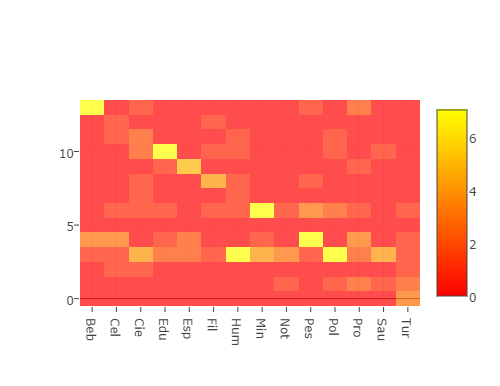
\includegraphics[width=0.9\textwidth]{nb_apenas_com_o_texto.png}
	\caption{Heatmap da matriz de confus�o da Tabela \ref{tab:nb_apenas_com_o_texto}}
	\label{fig:nb_apenas_com_o_texto}
\end{figure}

Outras estat�sticas analisadas s�o as precis�es, as abrang�ncias e os f1scores para cada uma das classes, conforme relacionado na Tabela \ref{tab:nb_apenas_com_o_texto_prec_rec}.

\begin{table}[tph]
	\begin{center}
		\begin{tabular}{ c  c  c  c }
			\hline
			Classe & Precisao & Abrangencia & F1score \\
			\hline
			Bebes & 0.636364 & 0.636364 & 0.636364 \\
			Celebridade & 0.500000 & 0.125000 & 0.200000 \\
			Ciencia & 0.400000 & 0.153846 & 0.222222 \\
			Educacao & 0.571429 & 0.615385 & 0.592593 \\
			Esporte & 0.714286 & 0.555556 & 0.625000 \\
			Filmes & 0.571429 & 0.500000 & 0.533333 \\
			Humor & 0.500000 & 0.083333 & 0.142857 \\
			Minorias & 0.409091 & 0.642857 & 0.500000 \\
			Noticias & 1.000000 & 0.000000 & 1.000000 \\
			Pessoal & 0.600000 & 0.777778 & 0.677419 \\
			Politica & 0.535211 & 0.883721 & 0.666667 \\
			Propaganda & 0.000000 & 1.000000 & 0.000000 \\
			Saude & 0.142857 & 0.166667 & 0.153846 \\
			Turismo & 1.000000 & 0.333333 & 0.500000 \\
			Media Micro & 0.529101 & 0.529101 & 0.529101 \\
			Media Macro & 0.541476 & 0.462417 & 0.498833 \\
			\hline
		\end{tabular}
	\end{center}
	\caption{Precis�o e abrangencia para NB apenas com o texto}
	\label{tab:nb_apenas_com_o_texto_prec_rec}
\end{table}


\section{Na�ve Bayes com Features Adicionais}
% Isso piora o classificador pois adiciona redundancia (e quebra a nocao de independencia condicional)

% citar a secao que explica essas features

A acur�cia m�dia obtida depois da adi��o das features extras foi de 51.1\%. A m�trica Kappa foi de 42.5\%. Observa-se portanto que houve uma pequena melhora em rela��o as redes Bayesianas com o texto puro(o Kappa variou de 41.4\% para 42.5\%). 

O motivo da melhoria ser t�o pequena � que ocorrem dois efeitos opostos quando se adicionam essas novas features. Por um lado, essas novas features adicionam novas informa��es que possibilitam que haja uma melhor classifica��o. Por outro lado, essas novas features s�o muitas vezes dependentes condicionalmente das palavras do texto. Como as NB assumem, independ�ncia condicional, a adi��o de features dependentes pode piorar a rede. O resultado da soma desses dois efeitos foi ligeiramente positivo neste caso.

A Figura \ref{fig:nb_features_extras_accuracy_graph} abaixo mostra a evolu��o da acur�cia das NB com features extras em fun��o do tamanho da base de dados. A Figura \ref{fig:nb_features_extras_kappa_graph} mostra a rela��o do Kappa com o tamanho da base de dados. A Figura \ref{fig:nb_features_extras_vs_apenas_texto_kappa_graph} compara os gr�ficos do Kappa para as NB com e sem features extras.

\begin{figure}[ht!]
	\centering	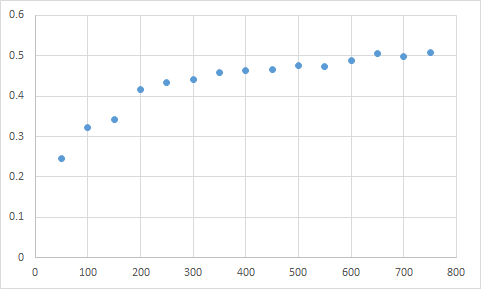
\includegraphics[width=0.9\textwidth]{nb_features_extras_accuracy_graph.png}
	\caption{Acur�cia em fun��o da quantidade de postagens na base de dados (treinamento + valida��o) para NB com features extras (alem das palavras do texto)}
	\label{fig:nb_features_extras_accuracy_graph}
\end{figure}


\begin{figure}[ht!]
	\centering	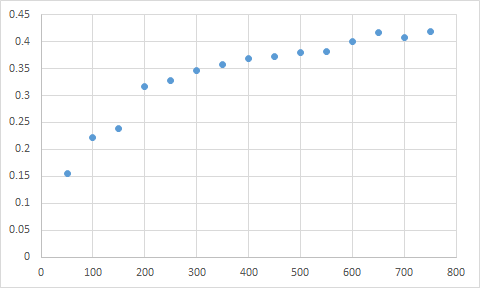
\includegraphics[width=0.9\textwidth]{nb_features_extras_kappa_graph.png}
	\caption{Kappa em fun��o da quantidade de postagens na base de dados (treinamento + valida��o) para NB com features extras (alem das palavras do texto)}
	\label{fig:nb_features_extras_kappa_graph}
\end{figure}

\begin{figure}[ht!]
	\centering	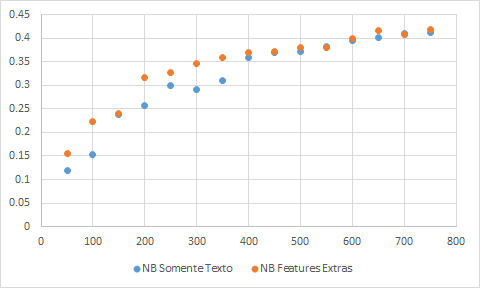
\includegraphics[width=0.9\textwidth]{nb_features_extras_vs_apenas_texto_kappa_graph.png}
	\caption{Sobreposi��o dos gr�ficos do Kappa em fun��o da quantidade de postagens na base de dados para NB com e sem as features extras}
	\label{fig:nb_features_extras_vs_apenas_texto_kappa_graph}
\end{figure}

Para este exemplo tem-se:

$acuracia=0.513228$

$acuracia\_esperada=0.140058$

$Kappa=0.433948$


A Tabela \ref{tab:nb_com_features_adicionais} apresenta a matriz de confusao.


\begin{table}[tph]
	\begin{center}
		\begin{tabular}{ c  c  c  c  c  c  c  c  c  c  c  c  c  c }
			\hline
			Beb & Cel & Cie & Edu & Esp & Fil & Hum & Min & Not & Pes & Pol & Pro & Sau & Tur\\
			\hline
			6 & 0 & 0 & 0 & 0 & 0 & 1 & 0 & 0 & 0 & 0 & 0 & 0 & 1\\
			0 & 0 & 0 & 0 & 0 & 0 & 0 & 0 & 0 & 0 & 0 & 0 & 0 & 0\\
			0 & 1 & 3 & 0 & 0 & 1 & 0 & 0 & 1 & 0 & 0 & 1 & 1 & 0\\
			0 & 0 & 3 & 3 & 1 & 0 & 0 & 0 & 0 & 0 & 0 & 1 & 0 & 0\\
			0 & 0 & 0 & 0 & 1 & 0 & 0 & 0 & 0 & 0 & 0 & 0 & 0 & 0\\
			0 & 0 & 0 & 0 & 0 & 3 & 0 & 0 & 0 & 0 & 0 & 0 & 0 & 0\\
			0 & 0 & 0 & 0 & 0 & 0 & 5 & 0 & 0 & 0 & 0 & 0 & 0 & 0\\
			1 & 0 & 0 & 2 & 1 & 1 & 0 & 6 & 2 & 1 & 1 & 0 & 1 & 0\\
			0 & 0 & 0 & 0 & 0 & 0 & 0 & 0 & 0 & 0 & 0 & 0 & 0 & 0\\
			4 & 3 & 0 & 3 & 6 & 3 & 4 & 2 & 1 & 22 & 1 & 1 & 1 & 2\\
			0 & 2 & 2 & 4 & 1 & 2 & 2 & 5 & 5 & 2 & 39 & 0 & 7 & 0\\
			0 & 0 & 1 & 0 & 1 & 3 & 0 & 0 & 0 & 0 & 0 & 3 & 0 & 1\\
			0 & 0 & 0 & 0 & 0 & 0 & 0 & 0 & 0 & 0 & 1 & 0 & 2 & 0\\
			0 & 0 & 0 & 0 & 0 & 0 & 0 & 0 & 0 & 0 & 0 & 0 & 0 & 4\\
			\hline
		\end{tabular}
	\end{center}
	\caption{Matriz de confusao para a NB com features adicionais}
	\label{tab:nb_com_features_adicionais}
\end{table}


A Figura \ref{fig:nb_com_features_adicionais} consiste numa representa��o gr�fica da matriz de confus�o.

\begin{figure}[ht!]
	\centering	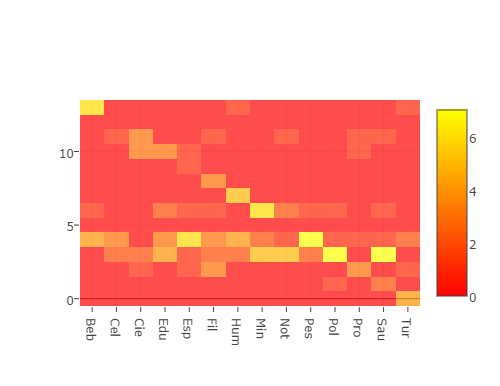
\includegraphics[width=0.9\textwidth]{nb_com_features_adicionais.png}
	\caption{Heatmap da matriz de confus�o da Tabela \ref{tab:nb_com_features_adicionais}}
	\label{fig:nb_com_features_adicionais}
\end{figure}

Outras estat�sticas analisadas s�o as precis�es, as abrang�ncias e os f1scores para cada uma das classes, conforme relacionado na Tabela \ref{tab:nb_com_features_adicionais_prec_rec}.

\begin{table}[tph]
	\begin{center}
		\begin{tabular}{ c  c  c  c }
			\hline
			Classe & Precisao & Abrangencia & F1score \\
			\hline
			Bebes & 0.750000 & 0.545455 & 0.631579 \\
			Celebridade & 1.000000 & 0.000000 & 0.000000 \\
			Ciencia & 0.375000 & 0.333333 & 0.352941 \\
			Educacao & 0.375000 & 0.250000 & 0.300000 \\
			Esporte & 1.000000 & 0.090909 & 0.166667 \\
			Filmes & 1.000000 & 0.230769 & 0.375000 \\
			Humor & 1.000000 & 0.416667 & 0.588235 \\
			Minorias & 0.375000 & 0.461538 & 0.413793 \\
			Noticias & 1.000000 & 0.000000 & 0.000000 \\
			Pessoal & 0.415094 & 0.880000 & 0.564103 \\
			Politica & 0.549296 & 0.928571 & 0.690265 \\
			Propaganda & 0.333333 & 0.500000 & 0.400000 \\
			Saude & 0.666667 & 0.166667 & 0.266667 \\
			Turismo & 1.000000 & 0.500000 & 0.666667 \\
			Media Micro & 0.513228 & 0.513228 & 0.513228 \\
			Media Macro & 0.702814 & 0.378850 & 0.492317 \\
			\hline
		\end{tabular}
	\end{center}
	\caption{Precis�o e abrangencia para NB com features adicionais}
	\label{tab:nb_com_features_adicionais_prec_rec}
\end{table}


\section{Weighted Na�ve Bayes utilizando apenas o texto}
%notar que apesar da acuracia ter melhorado pouco, o Kappa melhorou muito

A acur�cia m�dia obtida, depois da adi��o de pesos nas features e utilizando apenas as palavras do texto, foi de 53.5\%. A m�trica Kappa foi de 48.2\%. Observa-se portanto que houve uma melhora consider�vel na m�trica Kappa em rela��o �s abordagens anteriores e uma melhora pequena na acur�cia.

\begin{figure}[ht!]
	\centering	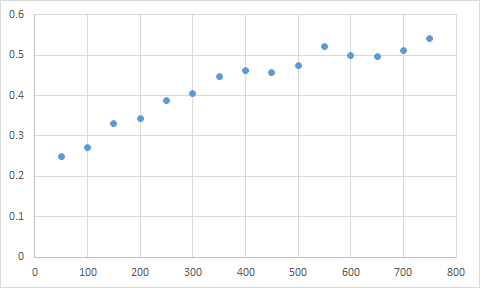
\includegraphics[width=0.9\textwidth]{wnb_somente_texto_accuracy_graph.png}
	\caption{Acur�cia em fun��o da quantidade de postagens na base de dados (treinamento + valida��o) para a Weighted NB utilizando apenas o texto}
	\label{fig:wnb_somente_texto_accuracy_graph}
\end{figure}


\begin{figure}[ht!]
	\centering	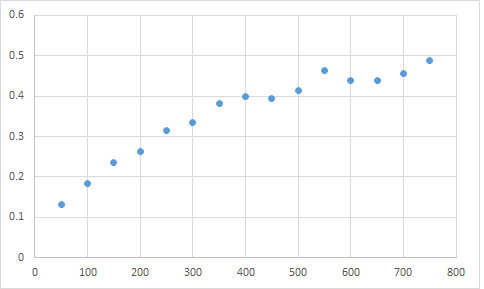
\includegraphics[width=0.9\textwidth]{wnb_somente_texto_kappa_graph.png}
	\caption{Kappa em fun��o da quantidade de postagens na base de dados (treinamento + valida��o) para a Weighted NB utilizando apenas o texto}
	\label{fig:wnb_somente_texto_kappa_graph}
\end{figure}

\begin{figure}[ht!]
	\centering	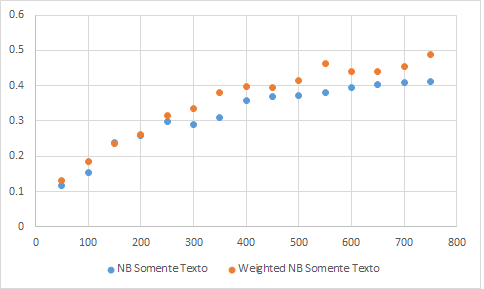
\includegraphics[width=0.9\textwidth]{nb_somente_texto_vs_wnb_kappa_graph.png}
	\caption{Sobreposi��o dos gr�ficos do Kappa em fun��o da quantidade de postagens na base de dados para o NB Simples e o Weighted NB}
	\label{fig:nb_somente_texto_vs_wnb_kappa_graph}
\end{figure}

Para este exemplo tem-se:

$acuracia=0.544974$

$acuracia\_esperada=0.104000$

$Kappa=0.492158$


A Tabela \ref{tab:weighted_nb_apenas_com_texto} apresenta a matriz de confusao.


\begin{table}[tph]
	\begin{center}
		\begin{tabular}{ c  c  c  c  c  c  c  c  c  c  c  c  c  c }
			\hline
			Beb & Cel & Cie & Edu & Esp & Fil & Hum & Min & Not & Pes & Pol & Pro & Sau & Tur\\
			\hline
			7 & 0 & 1 & 0 & 0 & 1 & 0 & 2 & 0 & 1 & 0 & 1 & 0 & 0\\
			0 & 1 & 0 & 0 & 1 & 0 & 0 & 0 & 0 & 0 & 0 & 0 & 0 & 0\\
			0 & 0 & 6 & 1 & 0 & 0 & 1 & 0 & 0 & 0 & 1 & 0 & 1 & 1\\
			1 & 0 & 3 & 8 & 1 & 0 & 0 & 1 & 0 & 0 & 2 & 1 & 2 & 0\\
			0 & 0 & 0 & 0 & 8 & 0 & 0 & 0 & 0 & 0 & 2 & 1 & 0 & 0\\
			0 & 1 & 0 & 0 & 0 & 12 & 0 & 0 & 0 & 1 & 2 & 1 & 0 & 2\\
			0 & 0 & 0 & 0 & 0 & 0 & 2 & 0 & 0 & 0 & 0 & 0 & 0 & 0\\
			2 & 1 & 1 & 1 & 0 & 0 & 2 & 9 & 1 & 4 & 12 & 0 & 0 & 2\\
			0 & 0 & 0 & 0 & 0 & 0 & 0 & 0 & 0 & 0 & 0 & 0 & 0 & 0\\
			1 & 0 & 0 & 0 & 2 & 0 & 1 & 1 & 0 & 12 & 0 & 0 & 0 & 1\\
			1 & 2 & 0 & 1 & 0 & 1 & 3 & 0 & 0 & 2 & 24 & 0 & 2 & 1\\
			0 & 0 & 0 & 1 & 0 & 1 & 1 & 1 & 0 & 0 & 1 & 3 & 0 & 0\\
			0 & 0 & 0 & 0 & 0 & 0 & 0 & 0 & 0 & 0 & 0 & 0 & 6 & 0\\
			0 & 0 & 0 & 1 & 1 & 0 & 0 & 0 & 0 & 0 & 1 & 0 & 0 & 5\\
			\hline
		\end{tabular}
	\end{center}
	\caption{Matriz de confusao para a Weighted NB apenas com texto}
	\label{tab:weighted_nb_apenas_com_texto}
\end{table}


A Figura \ref{fig:weighted_nb_apenas_com_texto} consiste numa representa��o gr�fica da matriz de confus�o.

\begin{figure}[ht!]
	\centering	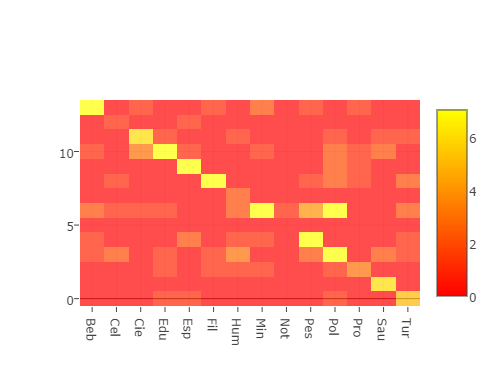
\includegraphics[width=0.9\textwidth]{weighted_nb_apenas_com_texto.png}
	\caption{Heatmap da matriz de confus�o da Tabela \ref{tab:weighted_nb_apenas_com_texto}}
	\label{fig:weighted_nb_apenas_com_texto}
\end{figure}

Outras estat�sticas analisadas s�o as precis�es, as abrang�ncias e os f1scores para cada uma das classes, conforme relacionado na Tabela \ref{tab:weighted_nb_apenas_com_texto_prec_rec}.

\begin{table}[tph]
	\begin{center}
		\begin{tabular}{ c  c  c  c }
			\hline
			Classe & Precisao & Abrangencia & F1score \\
			\hline
			Bebes & 0.538462 & 0.583333 & 0.560000 \\
			Celebridade & 0.500000 & 0.200000 & 0.285714 \\
			Ciencia & 0.545455 & 0.545455 & 0.545455 \\
			Educacao & 0.421053 & 0.615385 & 0.500000 \\
			Esporte & 0.727273 & 0.615385 & 0.666667 \\
			Filmes & 0.631579 & 0.800000 & 0.705882 \\
			Humor & 1.000000 & 0.200000 & 0.333333 \\
			Minorias & 0.257143 & 0.642857 & 0.367347 \\
			Noticias & 1.000000 & 0.000000 & 0.000000 \\
			Pessoal & 0.666667 & 0.600000 & 0.631579 \\
			Politica & 0.648649 & 0.533333 & 0.585366 \\
			Propaganda & 0.375000 & 0.428571 & 0.400000 \\
			Saude & 1.000000 & 0.545455 & 0.705882 \\
			Turismo & 0.625000 & 0.416667 & 0.500000 \\
			Media Micro & 0.544974 & 0.544974 & 0.544974 \\
			Media Macro & 0.638306 & 0.480460 & 0.548248 \\
			\hline
		\end{tabular}
	\end{center}
	\caption{Precis�o e abrangencia para Weighted NB apenas com texto}
	\label{tab:weighted_nb_apenas_com_texto_prec_rec}
\end{table}


\section{Weighted Na�ve Bayes com Features Adicionais}
% Nesse caso nao tem problema adicionar features redundantes pois os pesos aliviam a hipotese de independencia condicional

\begin{figure}[ht!]
	\centering	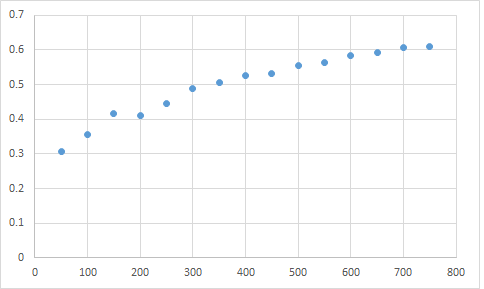
\includegraphics[width=0.9\textwidth]{wnb_features_extras_accuracy_graph.png}
	\caption{Acur�cia em fun��o da quantidade de postagens na base de dados (treinamento + valida��o) para a Weighted NB com features extras}
	\label{fig:wnb_features_extras_accuracy_graph}
\end{figure}


\begin{figure}[ht!]
	\centering	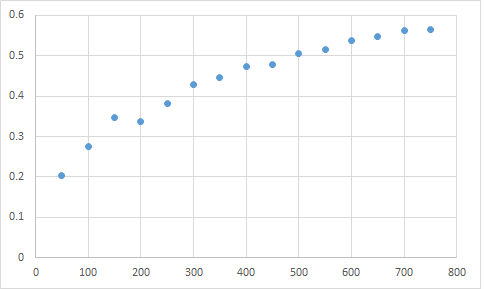
\includegraphics[width=0.9\textwidth]{wnb_features_extras_kappa_graph.png}
	\caption{Kappa em fun��o da quantidade de postagens na base de dados (treinamento + valida��o) para a Weighted NB com features extras}
	\label{fig:wnb_features_extras_kappa_graph}
\end{figure}

\begin{figure}[ht!]
	\centering	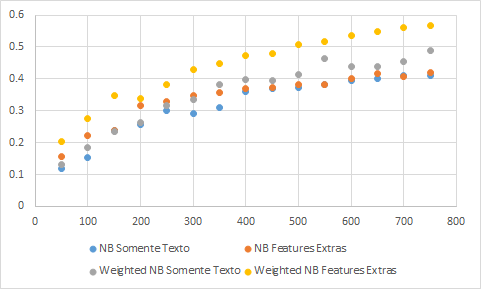
\includegraphics[width=0.9\textwidth]{nb_vs_wnb.png}
	\caption{Compara��o dos quatro classificadores propostos, mostrando o Kappa de cada um como uma fun��o do tamanho da base de dados.}
	\label{fig:nb_vs_wnb}
\end{figure}


Para este exemplo tem-se:

$acuracia=0.656085$

$acuracia\_esperada=0.108060$

$Kappa=0.614419$


A Tabela \ref{tab:weighted_nb_com_features_extras} apresenta a matriz de confusao.


\begin{table}[tph]
	\begin{center}
		\begin{tabular}{ c  c  c  c  c  c  c  c  c  c  c  c  c  c }
			\hline
			Beb & Cel & Cie & Edu & Esp & Fil & Hum & Min & Not & Pes & Pol & Pro & Sau & Tur\\
			\hline
			5 & 1 & 1 & 1 & 0 & 0 & 0 & 0 & 0 & 0 & 0 & 1 & 0 & 0\\
			0 & 3 & 0 & 0 & 0 & 0 & 0 & 0 & 0 & 0 & 0 & 0 & 0 & 0\\
			0 & 0 & 6 & 0 & 0 & 0 & 0 & 0 & 1 & 1 & 1 & 0 & 0 & 0\\
			0 & 0 & 5 & 7 & 1 & 1 & 0 & 3 & 0 & 0 & 4 & 1 & 1 & 0\\
			0 & 0 & 1 & 0 & 7 & 0 & 0 & 0 & 0 & 0 & 0 & 0 & 0 & 1\\
			0 & 0 & 0 & 1 & 0 & 7 & 0 & 0 & 0 & 0 & 0 & 1 & 1 & 0\\
			0 & 0 & 0 & 0 & 0 & 0 & 5 & 0 & 0 & 0 & 0 & 0 & 0 & 0\\
			2 & 1 & 0 & 0 & 0 & 0 & 0 & 14 & 2 & 0 & 5 & 0 & 1 & 0\\
			0 & 0 & 0 & 0 & 0 & 0 & 0 & 0 & 1 & 0 & 1 & 0 & 0 & 0\\
			2 & 1 & 0 & 0 & 0 & 0 & 0 & 1 & 0 & 24 & 1 & 2 & 0 & 2\\
			1 & 0 & 0 & 0 & 0 & 1 & 0 & 1 & 0 & 0 & 30 & 0 & 1 & 1\\
			0 & 0 & 1 & 1 & 0 & 1 & 0 & 0 & 0 & 1 & 1 & 4 & 0 & 0\\
			0 & 0 & 0 & 1 & 0 & 1 & 0 & 0 & 1 & 0 & 2 & 0 & 6 & 0\\
			0 & 1 & 0 & 0 & 0 & 0 & 0 & 0 & 0 & 0 & 0 & 0 & 0 & 5\\
			\hline
		\end{tabular}
	\end{center}
	\caption{Matriz de confusao para a Weighted NB com features extras}
	\label{tab:weighted_nb_com_features_extras}
\end{table}


A Figura \ref{fig:weighted_nb_com_features_extras} consiste numa representa��o gr�fica da matriz de confus�o.

\begin{figure}[ht!]
	\centering	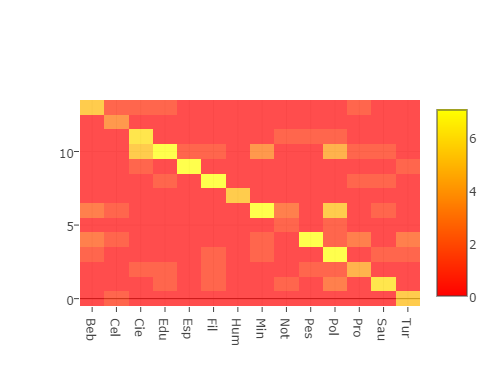
\includegraphics[width=0.9\textwidth]{weighted_nb_com_features_extras.png}
	\caption{Heatmap da matriz de confus�o da Tabela \ref{tab:weighted_nb_com_features_extras}}
	\label{fig:weighted_nb_com_features_extras}
\end{figure}

Outras estat�sticas analisadas s�o as precis�es, as abrang�ncias e os f1scores para cada uma das classes, conforme relacionado na Tabela \ref{tab:weighted_nb_com_features_extras_prec_rec}.

\begin{table}[tph]
	\begin{center}
		\begin{tabular}{ c  c  c  c }
			\hline
			Classe & Precisao & Abrangencia & F1score \\
			\hline
			Bebes & 0.555556 & 0.500000 & 0.526316 \\
			Celebridade & 1.000000 & 0.428571 & 0.600000 \\
			Ciencia & 0.666667 & 0.428571 & 0.521739 \\
			Educacao & 0.304348 & 0.636364 & 0.411765 \\
			Esporte & 0.777778 & 0.875000 & 0.823529 \\
			Filmes & 0.700000 & 0.636364 & 0.666667 \\
			Humor & 1.000000 & 1.000000 & 1.000000 \\
			Minorias & 0.560000 & 0.736842 & 0.636364 \\
			Noticias & 0.500000 & 0.200000 & 0.285714 \\
			Pessoal & 0.727273 & 0.923077 & 0.813559 \\
			Politica & 0.857143 & 0.666667 & 0.750000 \\
			Propaganda & 0.444444 & 0.444444 & 0.444444 \\
			Saude & 0.545455 & 0.600000 & 0.571429 \\
			Turismo & 0.833333 & 0.555556 & 0.666667 \\
			Media Micro & 0.656085 & 0.656085 & 0.656085 \\
			Media Macro & 0.676571 & 0.616533 & 0.645158 \\
			\hline
		\end{tabular}
	\end{center}
	\caption{Precis�o e abrangencia para Weighted NB com features extras}
	\label{tab:weighted_nb_com_features_extras_prec_rec}
\end{table}

\section{Utiliza��o dos links}
 
\section{Concatena��o do texto dos links}

\section{Fus�o de classes pequenas}

\section{Extens�o final desenvolvida}

\section{Teste de usabilidade}
% Usamos as heuristicas de Nielsen

\chapter{Conclus�es e Trabalhos Futuros}
\section{Conclus�es}

Este trabalho prop�s e analisou solu��es baseadas em Na�ve Bayes para se resolver o problema de classifica��o de postagens em redes sociais (especificamente no Facebook). Foram estudadas formas de se aliviar as considera��es de independ�ncia condicional, fazendo uso de pesos para as caracter�sticas.

Os resultados finais obtidos mostraram a viabilidade de se realizar este tipo de classifica��o, uma vez que foi poss�vel obter acur�cias superiores a 60\% (com F1score macro tamb�m superior a 60\%) utilizando-se uma base de dados relativamente pequena. Um aumento consider�vel na base de dados melhoraria muito a performance obtida.

Muitos dos erros cometidos pelo classificador final s�o justific�veis por terem ocorrido em postagens que na pr�tica poderiam pertencer a mais de uma classe. Deste modo, como trabalho futuro prop�e-se a realiza��o de um estudo semelhante com classificadores do tipo \emph{multi-class / multi-label}.

\section{Trabalhos Futuros}

\begin{itemize}
	\item \textbf{Aumentar a base de dados}\\
		Conforme os gr�ficos mostram, acredita-se que aumentando a base de dados os resultados melhorar�o. Para realizar isso pode-se executar o \emph{Crawler} mais vezes para obter mais dados e divulgar o plugin para mais pessoas e, assim, conseguir mais exemplos.
	\item \textbf{Utilizar \emph{Multi-class / Multi-label}}\\
		Muitos posts podem ser considerados como pertencendo a mais de uma categoria, o que indica que utilizando \emph{Multi-class / Multi-label} a qualidade do classificador possa aumentar significativamente.
	\item \textbf{Utilizar mais caracter�sticas da rede social}\\
		Foram utilizadas algumas caracter�sticas como autor do post, se � publicidade ou n�o, etc. Por�m ainda h� bastantes caracter�sticas que poderiam ser utilizadas, como, por exemplo, quem comentou em determinado post, o pr�prio texto dos coment�rios, entre outros.
		Um ponto interessante � que foi utilizado apenas o autor dos posts como caracter�stica, contudo, seria poss�vel aprofundar as informa��es sobre o autor de forma a capturar um pouco a estrutura da pr�pria rede social, como por exemplo quem s�o os amigos do autor, de quais grupos ele pertence, assim em diante.
	\item \textbf{Utilizar Informa��o M�tua para reconhecimento de novas classes}\\
		Outra sugest�o � utilizar o conceito de Informa��o M�tua para cria��o de novas classes sob o escopo do usu�rio. Se alguns dos posts do usu�rio fa�am com que a Informa��o M�tua entre duas classes seja grande isso talvez signifique que uma nova classe derivada seja melhor, como por exemplo os t�picos Sa�de e Engenharia para alguns posts pudessem ser substitu�dos por Bio-tecnologia.
		\item \textbf{Utilizar Informa��o M�tua para classes com poucos exemplos}\\
		Enquanto uma classe n�o atinja n�mero de exemplos significativo (que � obtido por meio do plugin sendo utilizado por "supervisores") pode-se utilizar a classe entre cuja Informa��o M�tua seja maior para efeitos de classifica��o de novos posts para n�o degradar a qualidade. Uma vez atingido um n�mero m�nimo de exemplos passa-se a utilizar a pr�pria classe.
\end{itemize}

% TODO: [minor] Ajeitar as imagens float, as forcando a ficar na secao certa

\bibliography{referencias}
\bibliographystyle{plain}

% TODO: [minor] Completar folha registro documento e ajeitar o page para o certo
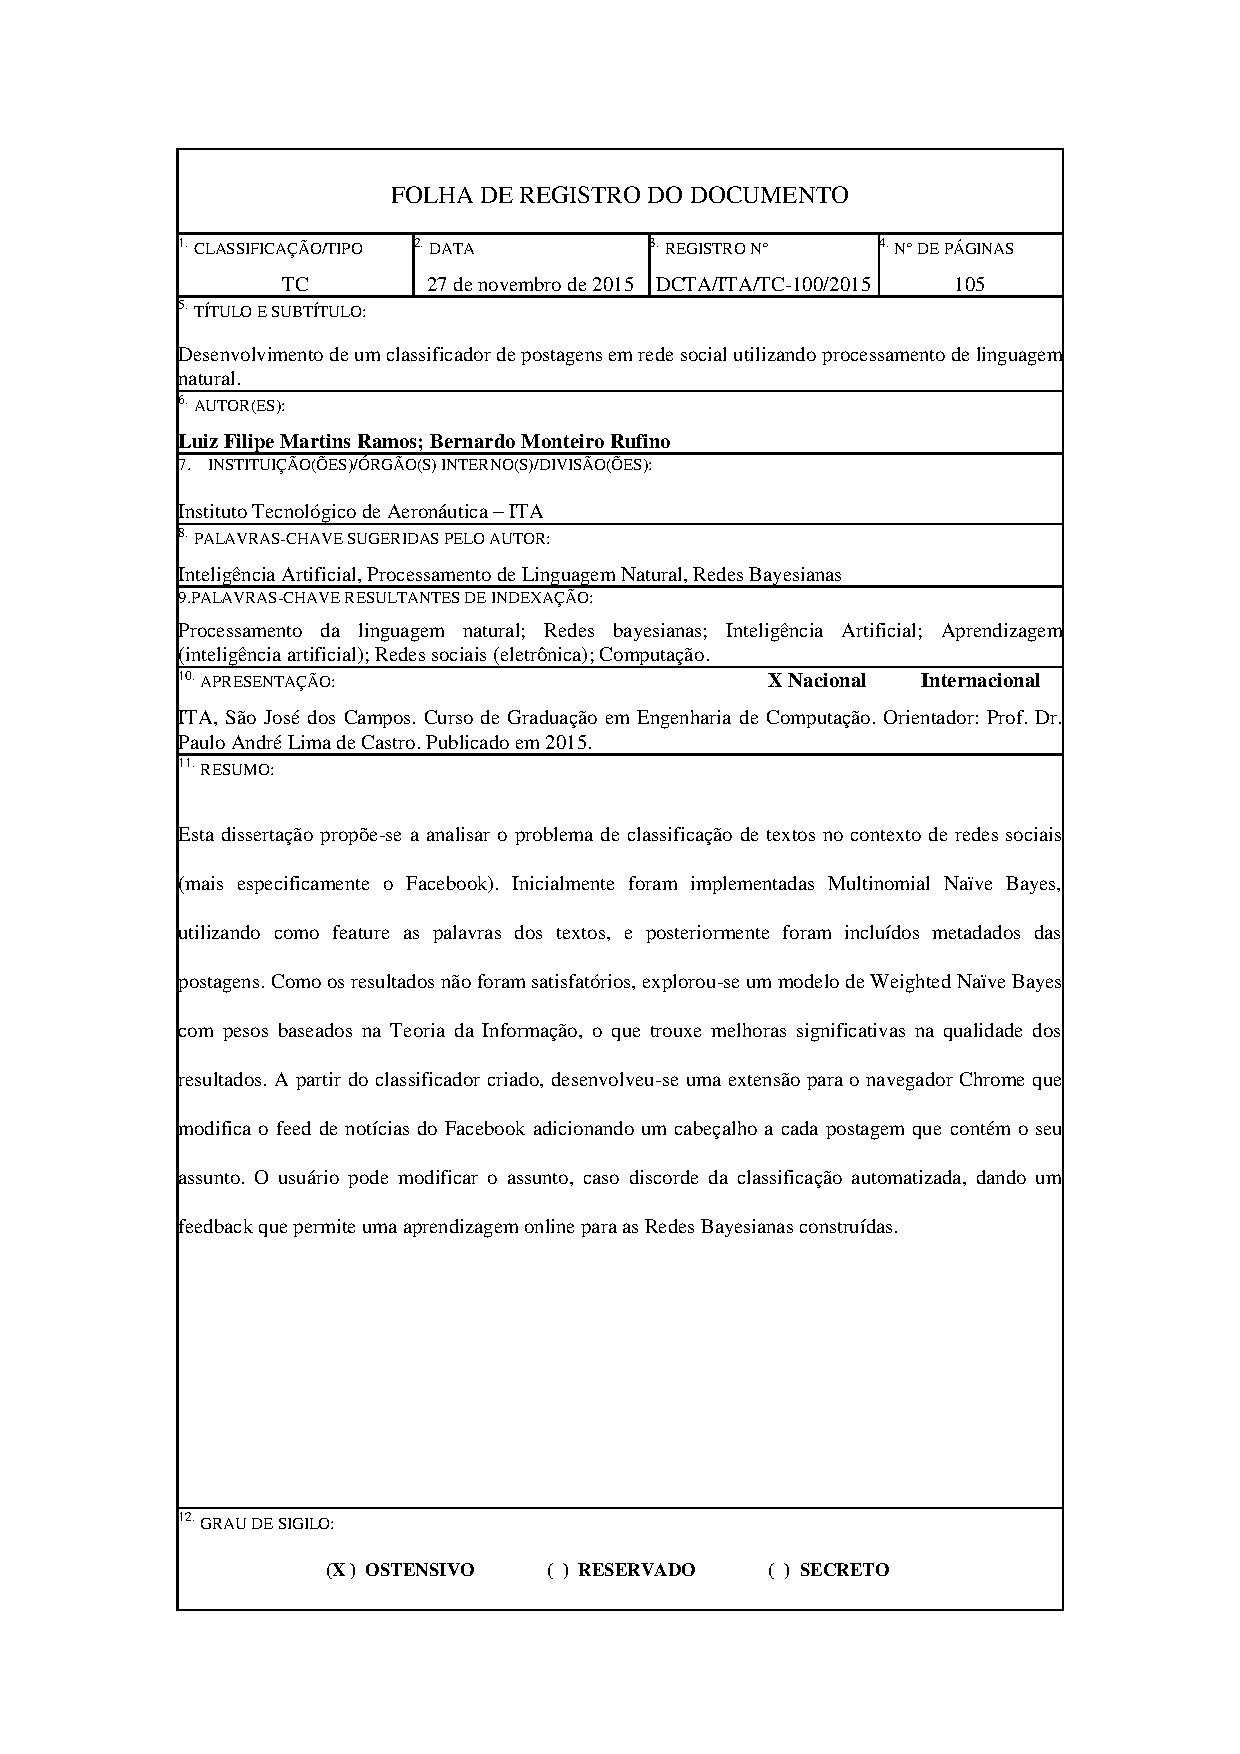
\includepdf{folha_registro_documento.pdf}
\bookmark[level=0, page=81]{Folha de Registro do Documento}

\end{document}